%%
%% GMU LaTeX MS Thesis Format Template
%%
%% Developed by:
%%      Daniel O. Awduche and Christopher A. St. Jean
%%      Communications and Networking Lab
%%      Dept. of Electrical and Computer Engineering
%%
%% Notes on usage can be found in the accompanying USAGE_NOTES.txt file.
%%
%%**********************************************************************
%% Legal Notice:
%% This code is offered as-is without any warranty either
%% expressed or implied; without even the implied warranty of
%% MERCHANTABILITY or FITNESS FOR A PARTICULAR PURPOSE!
%% User assumes all risk.
%% In no event shall any contributor to this code be liable for any damages
%% or losses, including, but not limited to, incidental, consequential, or
%% any other damages, resulting from the use or misuse of any information
%% contained here.
%%**********************************************************************
%%
%% $Id: GMU_thesis_template.tex,v 1.16 2007/05/02 02:20:11 Owner Exp $
%%

\documentclass[11 pt]{report}

%%  The file ``gmuthesis.sty''  is the GMU latex style file and
%%   should be placed in the same directory as your LaTeX files
\usepackage{gmuthesis}

%%
%% other packages that need to be loaded
%%
\usepackage[activate=true]{microtype} %don't hyphenate everywhere
\usepackage{graphicx}                    %   for imported graphics
\usepackage{rotating} %to rotate figs
\usepackage{amsmath}                     %%
\usepackage{amsfonts}                    %%  for AMS mathematics
\usepackage{amssymb}                     %%
\usepackage{amsthm}                      %%
\usepackage[normalem]{ulem}              %   a nice standard underline package
\usepackage[noadjust,verbose,sort]{cite} %   arranges reference citations neatly
\usepackage{setspace}                    %   for line spacing commands
\usepackage{float}                       %for precise placemnt of figs
\usepackage{subcaption} \usepackage{caption}
\usepackage{algorithmic} \usepackage{algorithm}
\usepackage{csvsimple}
\usepackage{hyperref}
\usepackage{enumitem}
% circled numbers for footnotes b/c it's confusing in math
\usepackage{pifont}
\renewcommand\thefootnote{\ding{\numexpr171+\value{footnote}}}
%for thick vertical line
\usepackage{array} \usepackage{makecell}
\usepackage[]{minted}
%http://tex.stackexchange.com/questions/237075/minted-not-working
%http://tex.stackexchange.com/questions/211672/cannot-get-tex-command-extra-options-to-work-in-auctex-11-88
\usepackage[table]{xcolor}

%% The file ``mythesisabbrev.sty'' is an (optional) personalized file that
%% may contain any and all LaTeX command (re)definitions that will be used
%% throughout the document
\usepackage{etoolbox}  \usepackage{mdframed}
\BeforeBeginEnvironment{minted}{\ls{1} \begin{mdframed}}%
\AfterEndEnvironment{minted}{\end{mdframed} \doublespacing}% ugly


\usepackage{amsmath,amssymb}
%matrix
\newcommand{\mt}[1]{\ensuremath{\mathbf{#1}}}
%vector
\newcommand{\vc}[1]{\ensuremath{\boldsymbol{#1}}}
%set
\newcommand{\st}[1]{\ensuremath{\mathcal{#1}}}
%time index
\newcommand{\tm}[1]{\ensuremath{\sp{(#1)}}}


%x
\newcommand{\x}[0]{\ensuremath{\vc{x}}}
%s
\newcommand{\s}[0]{\ensuremath{\vc{s}}}
%W
\newcommand{\W}[0]{\ensuremath{\mt{W}}}



% % fig stuff does not work!
% \usepackage{standalone}
% \usepackage{pgf}
% \usepackage{tikz}

%so that i can have a standlone cv
\usepackage{standalone}
\usepackage{pdfpages}

\beforedoc

\usepackage{caption}
\captionsetup[subfigure]{labelformat=simple}
\renewcommand{\thesubfigure}{(\alph{subfigure})}
\renewcommand{\subfigurename}{Figure \thefigure}

\begin{document}

%% In this section, all of the user-specific fields to be used in the
%% title pages are set
\title{%
  Unsupervised Anomaly Detection in Sequences\\
  Using Long Short Term Memory \\
  Recurrent Neural Networks} %todo ok title? recurrent is redundant!
\onelinetitle{%
  Unsupervised Anomaly Detection in Sequences
  Using Long Short Term Memory 
  Recurrent Neural Networks
} %todo ok title?
\author{%
Majid S. alDosari
}
\degree{Master of Science}
\subject{Computational Science}
\doctype{Thesis}
\dept{Computational and Data Sciences}
\degreeyear{2016}


\firstdeg{Bachelor of Science}
\firstdegschool{Vanderbilt University}
\firstdegyear{2003}
\seconddeg{Master of Science}
\seconddegschool{Vanderbilt University}
\seconddegyear{2012}


% Note: semester name should be written in its full-form. For example, Fall Semester, not just Fall.
\degreesemester{Spring Semester}

\advisor{Dr. Kirk D. Borne} %todo: middle inital?
\firstmember{Dr. Estela Blaisten-Barojas}
\secondmember{Dr. Igor Griva} 
\depthead{Dr. Kevin Curtin (acting)}
\assocdean{Dr. Donna Fox}
\dean{Dr. Peggy Agouris}


%%
%% Introductory pages
%%

% Note: The signature sheet is set according to the requirements of the Volgenau School of
% Information Technology and Engineering. If your college/school requirement is different,
% please make appropriate changes in the "signaturepage" section of gmudissertation.sty file.
\signaturepage



\titlepage

% copyright technically optional but should be included in to avoid potential pagination problems
\copyrightpage

%%
%% Dedication page
%%

\dedicationpage

\noindent I dedicate this thesis to my father, Saad F. al-Dosari, who supported me in this endeavor.

%%
%% Acknowledgements
%%

\acknowledgementspage

\noindent
I appreciate Dr. Borne's lead, as well as encouraging enthusiasm, in this endeavor.
%
Similarly, I am grateful to my other committee members, Dr. Blaisten-Barojas and Dr. Griva, who have given their time and input so that I may successfully complete my thesis.
%
Also, I give special thanks to John Kaufhold of Deep Learning Analytics for being responsive to my questions regarding anything related to neural networks.
%
His interest in and support of my work motivated me to do the best job that I can.
%
Last but not least, I appreciate very much that Leif Johnson, author of the \textsf{Theanets} neural network package that I used, provided assistance beyond user support.


%%
%% Table of contents, list of tables, and lists of figures
%%

\tableofcontents

\listoftables

\listoffigures



%%
%% Abstract
%%
\abstractpage

Long Short Term Memory (LSTM) recurrent neural networks (RNNs) are evaluated for their potential to generically detect anomalies in sequences.
%
First, anomaly detection techniques are surveyed at a high level so that their shortcomings are exposed.
%
The shortcomings are mainly their inflexibility in the use of a context `window' size and/or their suboptimal performance in handling sequences.
%
Furthermore, high-performing techniques for sequences are usually associated with their respective knowledge domains.
%
After discussing these shortcomings, RNNs are exposed mathematically as generic sequence modelers that can handle sequences of arbitrary length.
%
From there, results from experiments using RNNs show their ability to detect anomalies in a set of test sequences.
%
The test sequences had different types of anomalies and unique normal behavior.
%
Given the characteristics of the test data, it was concluded that the RNNs were not only able to generically distinguish rare values in the data (out of context) but were also able to generically distinguish abnormal \emph{patterns} (in context).

\abstractmultiplepage
In addition to the anomaly detection work, a solution for reproducing computational research is described.
%
The solution addresses reproducing compute applications based on \textsf{Docker} container technology as well as automating the infrastructure that runs the applications.
%
By design, the solution allows the researcher to seamlessly transition from local (test) application execution to remote (production) execution because little distinction is made between local and remote execution.
%
Such flexibility and automation allows the researcher to be more confident of results and more productive, especially when dealing with multiple machines.

%% Be sure to leave a line of whitespace immediately before this line!!!!!
%% (If this comment segment runs together with the preceeding text, you might
%%  see the second page of the abstract numbered "0".)
%%
%% If the abstract is more than one page, then place this line PRECISELY
%% at the page break; otherwise, comment it out.  (See note about this line
%% in the usage notes.)
%%
%\abstractmultiplepage
%The second page of the abstract
%%
%%  the main body of the dissertation
%%
\startofchapters
%% include the chapters one by one (or paste the chapter text in directly if desired)
\chapter{Introduction}
\label{ch:intro}

In the modern world, large amounts of time series%
\footnote{
In this document, the terms `time series' and `sequence' are used interchangeably without implication to the discussion.
%
Strictly however, a time series is a sequence of time-indexed elements.
%
So a sequence is the more general object.
%
As such, the term `sequence' is used when a general context is more applicable.
%
Furthermore, the terms do not imply that the data are real, discrete, or symbolic.
%
However, literature frequently uses the terms `time series' and `sequence' for real and symbolic data respectively.
%
Here, the term `time series' was used to emphasize that much data is recorded from monitoring devices which implies that a timestamp is associated with each data point.}
data of various types are recorded.  Inexpensive and compact instrumentation and storage allows various types of processes to be recorded. For example, human activity being recorded includes physiological signals, automotive traffic, website navigation activity, and communication network traffic. Other kinds of data are captured from instrumentation in industrial processes, automobiles, space probes, telescopes, geological formations, oceans, power lines, and residential thermostats. Furthermore, the data can be machine generated for diagnostic purposes such as web server logs, system startup logs, and satellite status logs.

Increasingly, these data are being analyzed. Inexpensive and ubiquitous networking has allowed the data to be transmitted for processing. At the same time, ubiquitous computing has allowed the data to be processed at the location of capture.

While the data can be recorded for historical purposes, much value can be obtained from finding anomalous data. However, it is challenging to manually analyze large and varied quantities of data to find anomalies. Even if a procedure can be developed for one type of data, it usually cannot be applied to another type of data.

Hence, the problem that is addressed can be stated as follows: find anomalous points in an arbitrary (unlabeled) sequence. So, a solution must use the same procedure to analyze different types of time series data.

The solution presented here comes from an unsupervised use of recurrent neural networks. A literature search only readily gives two similar solutions. In the acoustics domain, \cite{Marchi2015} transform audio signals into a sequence of spectral features which are then input to a denoising recurrent autoencoder. Improving on this, \cite{Malhotra2015} use recurrent neural networks (directly) without the use of features (that are specific to a problem domain, like acoustics) to multiple domains.

This work closely resembles \cite{Malhotra2015} but presenting a single, highly-automated procedure that applies to many domains is emphasized. First, some background is given on anomaly detection\footnote{Outlier, surprise, novelty, and deviation detection are alternative names used in literature.} that explains the challenges of finding a solution. Second, recurrent neural networks are introduced as general sequence modelers. Then, experiments will be presented to show that recurrent neural networks can find different types of anomalies in multiple domains. Finally, concluding remarks are given.

%todo pcc project

%%% Local Variables:
%%% mode: latex
%%% TeX-command-extra-options: "-shell-escape"
%%% TeX-master: "thesis"
%%% End:

%% chapter was hard to write b/c
% - survery of surveys 
% - conflicting information
% - little indication of what method to use for what kind of data
\chapter{The Challenge of Anomaly Detection in Sequences}
\label{ch:ad}

\section{Introduction}

The goal of this chapter is to show that the solution to the general problem of anomaly detection in time series is difficult. A typical general framework for anomaly detection in time series is explained with two advanced solutions as examples and their issues. The proposed solution, explained later in Chapter \ref{ch:results}, fits into the framework providing a basis for comparison.

Describing the variety of solutions puts the difficulty of finding a general solution in context. Furthermore, few publications survey the problem of anomaly detection for time series in particular \cite{Cheboli2010,Gupta2013}.

Solutions have been fragmented across a variety of application domains such as communication networks \cite{Jiang2006, Szymanski2004, Ye2000, Portnoy2001, Zhen2006, Warrender1999, Angiulli2007, Lane1999, Lane1997, Hofmeyr1998, Sequeira2002}, economics \cite{gupta2012community, Otey2006, Zhu2003}, environmental science \cite{Hill2010, Hill2010a, Angiulli2007, Birant2006, Cheng2006, Yuxiang2005, Wu2010, Drosdowsky1993, Lasaponara2006, Lu2004}, industrial process \cite{Basu2007, Nairac1999, Dasgupta1996, Bu2007}, biology \cite{Keogh2005, Wei2006}, astronomy \cite{Keogh2005, Yankov2008}, and transportation \cite{Li2009,Ge2010}. The fragmentation of application domains led to a variety of problem formulations \cite{Gupta2013}. Furthermore, there is no good understanding of how the solutions in different application domains compare to each other \cite{Cheboli2010}. Therefore, it is difficult to generalize the performance of a solution formulated in one application domain to its performance in another although they might have some commonalities.

Furthermore, adding to the difficulty of comparing solutions, the mechanics of anomaly detection have come from two disciplines with different priorities: statistics and computer science. Solutions from statistics focus on mathematical rigor while solutions from computer science consider computational issues \cite{Gupta2013}.


\cite{Gupta2013} offers a survey of anomaly detection solutions in a variety of settings such as streaming data, distributed data, and databases. But to focus the solution presented here, the problem will be stated as follows: Given a finite time series
 $\x$,
%
\begin{gather*}
\x=\{\x\tm{1},\x\tm{2},\x\tm{t},\ldots,\x\tm{T}\} \\
\x\tm{t} \in \mathbb{R}^v
,
\end{gather*}%
%
find points which can be considered anomalous where $T$ is the length of the regularly spaced sequence in time%
\footnote{Irregularly-spaced sequences might need a specific treatment. Of course, $\x$ can be treated as a sequence not indexed by time provided that some coherence is revealed over the index.}%
, $t$, and $v$ is the number of variables of $\x$. This statement is sensible only when anomalous points are a small part of the data. Furthermore, anomalies may not even be present.

So elements of any solution to this problem must answer the following questions:

\begin{enumerate}
\item
What is normal (as an anomaly is defined as what is \textit{not} normal)?
\item
What measure is used to indicate how anomalous point(s) are?
\item
How is the measure tested to decide if it is anomalous?
\end{enumerate}



\section{Anomaly Types}
\label{sec:anomalytypes}

The presence of different anomaly types can be a challenge for anomaly detection techniques. What follow are qualitative descriptions of anomalies classified in a way most relevant to this work. However, a taxonomy of anomalies will never encompass all anomalies as well as defining anomalies as points that are not normal.

\subsection{Point Anomalies}

Point anomalies are single points of interest that can be classified as follows.

\textbf{Simple:} Simple point anomalies are just defined by their value. They are trivial to describe and detect. They are not of much interest in themselves but are mentioned because anomalies in more complicated time series can be `converted' to resemble this simple type.

\begin{figure}[H]
  \centering
  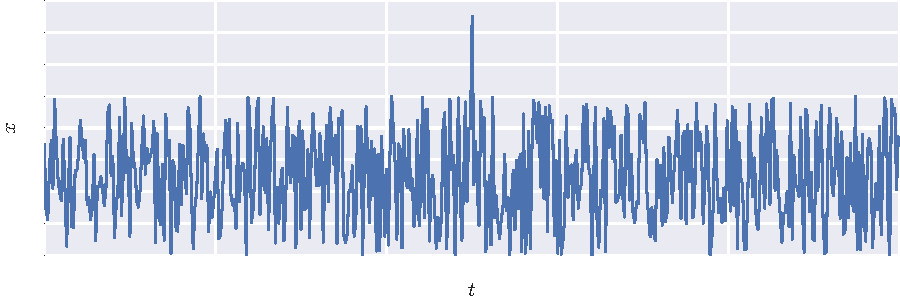
\includegraphics{figs/trivial.pdf}
  \caption{Simple point anomaly}
\end{figure}


\textbf{Context:} Some point anomalies are defined within a context. In Figure \ref{fig:contextanom}, the anomalous point's value is within the range of typical values. But if the cyclic nature of the series were removed, the anomaly is readily detected (`converted' to a simple point anomaly).

\begin{figure}[H]
  \centering
  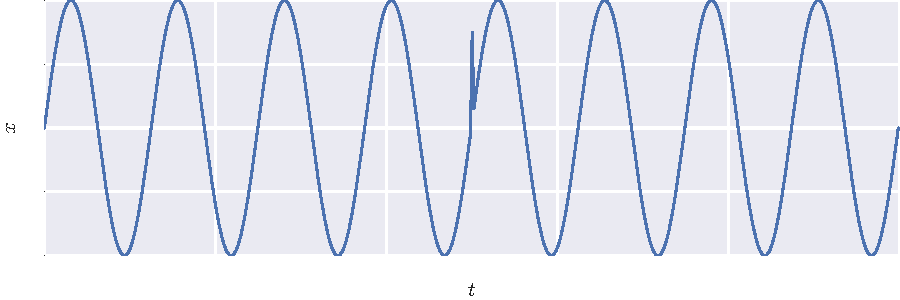
\includegraphics{figs/context.pdf}
  \caption{Anomaly in a periodic context}
  \label{fig:contextanom}
\end{figure}


\subsection{Discord}

Anomalies over subsequences are called discords \cite{Cheboli2010}. In Figure \ref{fig:perdiscordanom}, about two cycles in a periodic time series are unlike the other cycles. The repeated units do not have to be periodic as in Figure \ref{fig:aperdiscordanom}.

\begin{figure}[H]
  \centering
  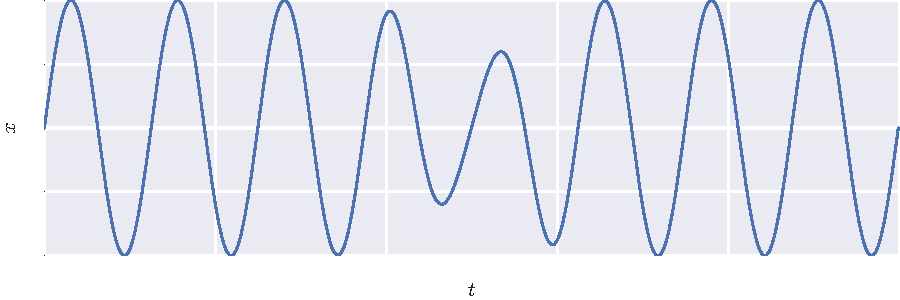
\includegraphics{figs/discord_per.pdf}
  \caption{Discord anomaly in a periodic time series}
  \label{fig:perdiscordanom}
\end{figure}

\begin{figure}[H]
  \centering
  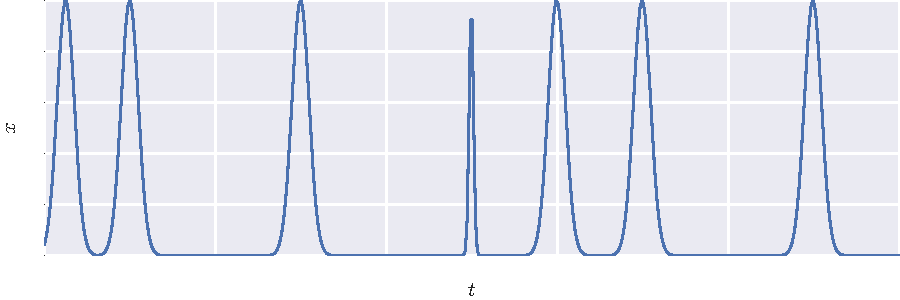
\includegraphics{figs/discord_aper.pdf}
  \caption{Discord anomaly in an aperiodic time series}
  \label{fig:aperdiscordanom}
\end{figure}

\subsection{Multivariate}

Multivariate\footnote{In this text, dimensionality of the time series will refer to the length of the time series as opposed to the number of its variables. Time series anomaly detection literature is inconsistent in the terminology used to refer to these two attributes.} time series add another element of complication for detecting anomalies in them and are not a focus in this work. \cite{Cheboli2010} classifies multivariate time series according to a combination of periodicity and synchronicity: Variables in a time series can be synchronous and periodic, synchronous and aperiodic, asynchronous and periodic, asynchronous and aperiodic. Therefore, any deviation from these properties are anomalies.




\section{Procedure}


In this section, a procedure to find anomalies in time series will be outlined to help answer the questions posed in the introduction of this chapter. The focus will be on issues related to time series as opposed to the general anomaly detection problem. However, there will be a focus on the issues related to solving the general problem of finding anomalies in (an arbitrary) time series as opposed to finding anomalies in a particular application domain. But computational issues will not be emphasized.

By examining many detection techniques, a general procedure (Section 2.7 in \cite{Cheboli2010}) can be gleaned:

\begin{enumerate}
\item Compute an anomaly score for an observation (a point or a subsequence in a time series). The anomaly score is a deviation from some `normal' value such as the prediction from a model or similarity to other observations.
\item Aggregate the anomaly scores for many observations.
\item Use the anomaly scores to determine whether an observation can be considered anomalous. For example, an observation could be considered anomalous if its anomaly score exceeds three standard deviations from the mean of the anomaly scores.
\end{enumerate}

At a high level, the procedure is rather straightforward. But, the process of finding what is normal is not. This section is devoted to explaining why finding anomalies in time series is particularly challenging. Addressing the stated problem, given an (single) arbitrary time series, the process of finding normal behavior involves the following steps:
\begin{enumerate}
\item Extract Samples
\item Transform Samples
\item Apply Detection Technique
\end{enumerate}

\subsection{Sample Extraction}
\label{sec:adsample}

Many instances of data are needed to inform what is normal. So, subsequences need to be extracted from a (long) sequence.

Samples can be extracted from a sliding a window over the time series. More precisely, beginning at step $t=0$, sliding a window of width $w$ over a time series $x$ of length $T$ one step at a time produces $p=T-w+1$ windows, $\mathcal{X}=\{W_1,W_2,\ldots,W_p\}$\footnote{In literature, this form corresponds to a time series database \cite{Gupta2013}}.

Now, $\mathcal{X}$ contains all possible subsequences of $\x$ of length $w$ and the value $p$ is typically not much less than $T$. Having many subsequences helps to localize the anomaly; so the window capturing the anomaly will have a higher anomaly score than adjacent windows.

But sometimes it is not desirable for computational reasons to process all subsequences. $p$ can be reduced by introducing a `hop', $h$, that skips $h$ steps when advancing the window from the previous one ($h=1$ gives all possible subsequences).

However, by introducing a large enough hop, anomalies could be missed. Consider the sequence \emph{abc\underline{c}abcabc}. The second \emph{c} is an anomaly. Now inspect the windows generated by various values of $h$ in Table \ref{tbl:hop}. The anomalous \emph{c} is captured in a window when $h$ is 1 or 2 but not when $h$ is 3 or 4. As a general rule, when $h=1$, an anomaly would never be missed. But when $h>1$, there is a chance that anomalies would be missed.

\begin{table}[h]
  \centering
  \begin{tabular}{|c|c|}
    \hline
    hop ($h$) & Ordered Windows \\
    \hline
    \hline
    1 & \emph{abc},
        \emph{bc\underline{c}}, 
        \emph{c\underline{c}a}, 
        \emph{cab},
        \emph{abc}, 
        \emph{bca},
        \emph{cab},
        \emph{abc} \\
    \hline
    2 & \emph{abc},
        \emph{c\underline{c}a},
        \emph{abc},
        \emph{cab} \\
    \hline
    3 & \emph{abc}, 
        \emph{cab},
        \emph{cab} \\
    \hline
    4 & \emph{abc}, 
        \emph{abc} \\
    \hline
  \end{tabular}
  \caption[Point anomalies in sliding windows of various hop sizes]{Point anomalies in sliding windows of width 3 for various hop sizes for the sequence \emph{abc\underline{c}abcabc} are underlined (The \emph{c} in the first \emph{cab} for $h=1$ cannot be considered anomalous because it is not in its context). From \cite{Cheboli2010}.}
  \label{tbl:hop}
\end{table}

\begin{sloppypar}% bc the seq was getting into the margin
Another issue that needs to be considered when working with windows is that the window size must be large enough to capture an anomaly. Consider the sequence \emph{aaabbbccc\underline{c}aaabbbcccaaabbbccc} where the fourth \emph{c} is anomalous. The window width must be at least 4 to capture the fourth \emph{c}. In other words, the window size must be on the order of the anomalous behavior.
\end{sloppypar}

Now given $\mathcal{X}$ for some $w$, the problem may be posed as a multidimensional anomaly detection problem. In this setting, assuming that $\x$ is univariate, samples of $\mathcal{X}$ correspond to $w$ dimensions. However, doing so largely ignores the temporal nature of $\x$. These issues will be discussed within the forthcoming parts of this chapter.

Finally, subsequent steps taken in the anomaly detection process may put restrictions on $h$ and $w$. For example, if the window size is too large, there may not be enough samples to properly apply an anomaly detection technique.

\subsection{Transformation}

Anomalies can be more easily detected if the time series are analyzed in a different representation. Usually these representations are of lower fidelity but capture the essential characteristics of the time series in certain cases. As a general example, a real-valued time series could be or should be discretized into a finite set of symbols or numbers to make use of techniques from bioinformatics. Or, it could be transformed into a different domain such as the frequency domain to make use of techniques from signal processing. As an added benefit, the tranformed time series need less computation given their reduced representation.

More specifically, the Symbolic Aggregate approXimation (SAX) \cite{Lin2007} is an example of time series discretization used to find anomalies in  \cite{Keogh2005}. While the Haar transform represents a transformation to the frequency domain for the same purpose in \cite{Bu2007,fu2006finding}.

However, as a transformation only captures the essential characteristics of a time series, more subtle anomalies could be lost in the transformation process. For example, the anomaly in Figure \ref{fig:contextanom} would be difficult to encode in terms of frequency because it is localized in time while oscillations (representing frequencies) are not.

Another issue to consider is the similarity of the arrangment of time series `points' (like elements of $\mathcal{X}$ in $\mathbb{R}^w$) in the transformed space to that of the original space. Some anomaly detection techniques rely on a certain distribution of points in a space. Suppose an anomaly detection technique works in $\mathbb{R}^w$ by identifying points that are far away from some normal cluster of points. This arrangement should also be present in the transformed space. Anomaly detection techniques that rely on spaces are introduced in Section \ref{sec:adproximity}.

However, a recent empirical study \cite{Wang2013} suggests that, in general, there is little to differentiate between numerous time series representations. Only spectral transformations applied to periodic series showed some advantage but only in certain cases.

\subsection{Detection Technique}

Choosing the anomaly detection technique is the final (involved) step in setting up an anomaly detection process. Detection techniques are discussed as a separate chapter to allow for more development.

\chapter{Detection Technique}
\label{ch:adtechnique}

The application of anomaly detection in a wide variety of domains has led to the development of numerous detection techniques. Each of these applications defines anomalies in a different way;  some  may only be interested in single anomalous points while others are more concerned about anomalous subsquences (discords). Furthermore, techniques are developed drawing on theory from statistics, machine learning, data mining, information theory, and spectral theory.

A highest-level categorization of these techniques could be as follows. The categories are not exhaustive but capture a wide variety of techniques discussed in literature.

\begin{description}

\item[Segmentation] In segmentation-based techniques, the time series is first split into homogeneous segments. Then a finite-state automation is trained to learn transition probabilities between segments. So, a segmented anomalous time series should not have high transition probability \cite{Salvador2005,mahoney2005trajectory,Chan2005}.

\item[Information Theory] Information-theoretic techniques quantify a notion of information content such as entropy. So, a point is considered an anomaly if its removal reduces the information content significantly \cite{Muthukrishnan2004,jagadish1999mining}. That is, anomalous points increase disorder, or require more information to be represented in the sequence.

\item[Proximity] Techniques based on proximity map time series onto a space. It is expected that anomalous time series are `different' because they are far from normal ones.

\item[Model] The difference between the (actual) values of a time series and its predicted values from a model indicate how anomalous they are.
 
\end{description}


Given the variety of techniques applied in different application domains, it is not always possible to use a solution developed for one problem and apply it to another. Finding a general anomaly detection technique is difficult. To the author's knowledge, only one study \cite{Cheboli2010} attempted to compare anomaly detection techniques over a wide variety of data. The study showed, as expected, varying performance of the techniques. A combination of time series characteristics and algorithm settings were sometimes used as explanations for the varying performance. These explanations do not help to objectively determine \emph{a priori} what technique to use and how to adjust any parameters it might use.

It would be difficult to use information theoretic techniques because finding an information theoretic measure sensitive enough to detect a few anomalies is challenging \cite{Chandola2009}. Segmentation-based techniques require that a time series to be made of homogeneous segments. These conditions are deemed too restrictive to be able to solve the general problem. In addition, both are not well-studied. So, they are not further explored here.

This leaves model-based techniques and proximity-based techniques as potential solution categories. Both are widely studied. Furthermore, it is possible to make a theoretical comparison between model-based techniques and proximity-based techniques if they are evaluated as, respectively, generative and discriminative models \cite{Ng2006}. Model-based techniques are usually preferred for anomaly detection \cite{Ngkvist2014} assuming enough training data are available.

Obviously, a good model is needed as well; recurrent neural networks will be introduced in the next chapter. However, proximity-based solutions are explored in this chapter as a benchmark for comparison as they are well-studied and have had numerous successful applications. Also, the hidden Markov model is introduced as an example of model-based solutions in this chapter as another benchmark.


\section{Proximity}
\label{sec:adproximity}

As previously mentioned, proximity-based techniques map time series as points of dimension $w$ in some space using some distance measure. The distance measure is used to evaluate how close a test time series is to others; anomalous time series are those that are far (dissimilar) from those considered normal.

This implies that the time series `points' are arranged in a certain way in the space. In two dimensions, the simplest distribution is portrayed in Figure \ref{fig:simple_dist}. Normal points, $\mathcal{N}_1$, are somewhat clustered. To test whether $p_1$ is an anomaly, it is easy to see, and calculate, that point $p_1$'s nearest neighbor is larger than the nearest neighbor distances of all other points.

\begin{figure}[H]
  \centering
  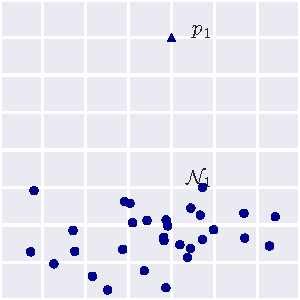
\includegraphics{figs/simple_dist.pdf}
  \caption{Simple anomaly distribution}
  \label{fig:simple_dist}
\end{figure}

Practically, this idealization never occurs. It is not as simple to objectively distinguish $p_1$ and $p_2$ from $\mathcal{N}_1$ and $\mathcal{N}_2$ in the situations depicted in Figure \ref{fig:hard_dist}.

\begin{figure}[H]
  \centering
  \begin{subfigure}[H]{2in}
    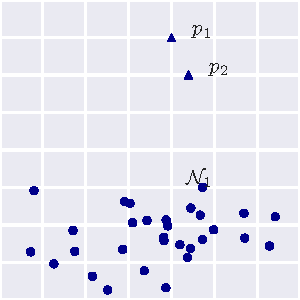
\includegraphics{figs/hard1_dist.pdf}
    \caption{}
    \label{fig:hard1_dist}
  \end{subfigure}
  \begin{subfigure}[H]{2in}
    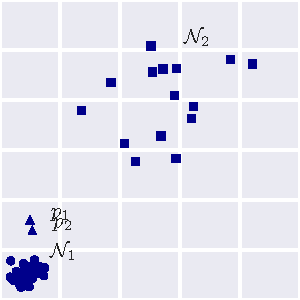
\includegraphics{figs/hard2_dist.pdf}
    \caption{}
    \label{fig:hard2_dist}
  \end{subfigure}
  \caption{Complex anomaly distribution}
  \label{fig:hard_dist}
\end{figure}


\subsection{Effects on Point Distribution}

Having complex distributions is the purview of anomaly detection in general and not a problem particular to time series data. However, issues influenced by the temporal nature of the data will be the focus of this subsection.

\subsubsection{Distance Measure}%

The choice of distance measure is crucial for anomaly detection because it captures some intuitive notion of similarity between a pair of time series. It is possible to use the `ordinary' Eucilidean distance \cite{Keogh2002} but it does not always capture the desired similarity between a pair of time series. The comparison between time series should be invariant to the following factors:

\begin{description}

\item[Length]  \hfill \\
%
Sometimes it is desirable to be able to compare sequences of different lengths. Compare the sequence, \emph{ababababab}, to a shorter one, \emph{abababa}. There is reason to believe that both are at least highly similar.

\item[Skew] \hfill \\
%
Consider the sequence \emph{abaababaaabaabab} and \emph{aaababaababaabab} where occurances of \emph{b} are padded by an unpredictable number of \emph{a}'s. The sequences can be considered similar even if they are not strictly periodic.

Dynamic Time Warping (DTW) \cite{Keogh2002} is capable of identifying similarity in such scenarios by `warping' the sequences to minimize dissimilarity (DTW is also capable of comparing sequences of different lengths).

\item[Translation] \hfill \\
%
Typically, sequences that are shifted in time are considered similar. For example, \emph{abababab} is similar to \emph{babababa}. Despite the sophistication of DTW, a warping transformation would not make these two sequences similar.  Cross-correlation is a similarity measure that can handle translations \cite{Protopapas2005}.

\item[Amplitude] \hfill \\
%
Sometimes it is desirable to ignore differences in amplitude if two time series are otherwise similar. Distance measures are usually sensitive to differences in amplitude unless the time series are normalized \cite{Keogh2002}. 

\end{description}

So simple measures, like the Euclidean distance, are not able to accommodate these factors. However, recently, in a comprehensive study of similarity measures, \cite{Wang2013} finds that, in large data sets, the clustering accuracy of `elastic' measures, such as DTW, converges with that of the Euclidean distance. Nonetheless, the advantage of using DTW, as well as other elastic measures, is maintained for smaller data sets.

Furthermore, in addition to addressing the previously mentioned factors, the distance measure must be compatible with the time series representation \cite{Chakrabarti2002}. So, for example, if a symbolic representation is used, then the distance measure must be appropriate for symbolic data.


\subsubsection{Window Width}

Section \ref{sec:adsample} introduced the use of sliding windows to extract samples of some width\footnote{Window `size' or `length' might also be used to refer to window width}, $w$. Here, the effect of the choice of $w$ will be explained when combined with a distance measure.

Also in Section \ref{sec:adsample}, it was mentioned that $w$ should be, at least, on the order of the length of the expected anomaly. But when $w$ is too large the distance measure becomes less effective at measuring similarity because the proportion of the anomalous subsequence becomes small compared to $w$. Furthermore, pairs of points become more equidistant in high-dimensional space \cite{Hinneburg2000,Beyer1999} which makes distinguishing between time series difficult (though this could be mitigated by using a dimension-reducing transformation \cite{Keogh2001}).


\subsubsection{Sliding Windows}
\label{sec:sliding}

The mere action of extracting samples with a \emph{sliding} window (with a small $h$, in contrast to non-overlapping windows) can have a profound effect on the distribution of the samples in the space. The effects challenge assumptions about the organization of (sliding window) points for the task of anomaly detection.

\cite{Keogh2005} demonstrates that anomalous anomalous points are not necessarily located in sparse space. Conversely, repeated patterns are not necessarily located in dense space \cite{kitaguchi2004extracting,Chiu2003,Bentley1997}.

Furthermore, in a paper challenging the status quo, \cite{Keogh2004} makes the bold claim that clustering of time series with sliding windows is meaningless. It found no similarity between clusters found with a sliding window ($h<<w$) and clusters found when the windows did not overlap ($h>w$) which invalidated the results of previously published papers per its argument. However, some constraints were identified that may allow some data sets to be clustered. But a decade later, the issue of clustering subsequences of time series is unresolved \cite{Zolhavarieh2014}.

These findings place restrictions on selecting a proximity-based anomaly detection algorithm.


\subsection{Data Classification}

In the following subsections, data classification techniques (that facilitate anomaly detection) will be discussed. The techniques are not particular to time series data. However, finding anomalous windows of time series data is referred to as `discord detection' in literature.

\subsubsection{Local versus Global Techniques}

First it is instructive make a general note about how they work regardless of how they are classified.

Proximity-based anomaly detection techniques can use a global context (of all) data points or a local context to test whether a point is an anomaly. Going back to Figure \ref{fig:simple_dist}, it was mentioned that it is trivial to find the anomalous point using all data points. However, in \ref{fig:hard2_dist}, it is not trivial to distinguish $p_11$ and $p_2$ as anomalous in this global view due to their proximity to $\mathcal{N}_1$. An anomaly detection approach that considers the (local) neighborhood of points $p_1$ and $p_2$ must be used.

\subsection{Nearest-Neighbor}

Nearest-neighbor techniques assume that normal points are in dense neighborhoods while anomalies are far from them.

In the beginning of Section \ref{sec:adproximity}, it was noted how simple it is to determine that point $p_1$ in Figure \ref{fig:simple_dist} is anomalous. However, given the discussion about sliding windows in Section \ref{sec:sliding}, it is not as straightforward when dealing with data points generated from sliding windows.

The problem comes from adjacent windows being close to each other in space. Consider the windows of width equal to 3 for the sequence \emph{abcabcXXXabcababc} \cite{Keogh2005} in Figure \ref{tbl:selfmatch}. Obviously, the subsequence \emph{XXX} stands out as the most anomalous after \emph{bab}. But \emph{XXX} has the nearest matches \emph{cXX} and \emph{XXa} one step away as can be seen in the subsequences generated by advancing a window on every step ($h=1$). This makes the subsequence \emph{bab} as more anomalous because is it different by two symbols from its nearest match \emph{aba}. In contrast, when examining windows with no overlap ($h=3$), \emph{XXX} is far from all other subsequences.

\begin{table}[h]
  \centering
  \begin{tabular}{|c||c|}
    \hline
    $h=1$ & $h=3$ \\
    \hline
    \hline
    \emph{abc} & \emph{abc} \\
    \emph{bca} & \\
    \emph{cab} & \\
    \hline
    \emph{abc} & \emph{abc} \\
    \emph{bcX} & \\
    \emph{cXX} & \\
    \hline
    \emph{XXX} & \emph{XXX} \\
    \emph{XXa} & \\
    \emph{Xab} & \\
    \hline
    \emph{abc} & \emph{abc} \\
    \emph{bca} & \\
    \emph{cab} & \\
    \hline
    \emph{aba} & \emph{aba} \\ 
    \emph{bab} & \\
    \emph{abc} & \\
    \hline
  \end{tabular}
  \caption[Neighbors of sliding windows]{Neighbors of sliding windows of sequence \emph{abcabcXXXabcababc}}
  \label{tbl:selfmatch}
\end{table}

However, it is still possible to use overlapping windows to find subsequences like \emph{XXX}. The solution proposed by  \cite{Keogh2005} is to use non-self matches. So when when calculating distances (similarity) to neighbors of \emph{XXX}, only those that are at least one window width away are considered. In this calculation, \emph{XXX} would not have any neighbors with the symbol \emph{X}.

Furthermore, the solution in \cite{Keogh2005} improves upon the brute force discord search by employing a heuristic called HOT SAX: Heuristically Ordered Time series using Symbolic Aggregate approXimation. But the time series is discretized as part of its process.

If the issues with sliding windows can be mitigated, it is possible to use anomaly detection techniques that are not specific to time series. Nearest-neighbor techniques can use either the $k$th nearest neighbor (kNN) distance or the relative density of a region around a point in the calculation of its anomaly score.

For example, the kNN distance can be used to identify that $p_1$ and $p_2$ are anomalies in Figure \ref{fig:hard1_dist}. By choosing, say, $k=4$, the fourth nearest neighbor of points $p_1$ and $p_2$ would be a point in \emph{far} away in $\mathcal{N}_1$. While the fourth nearest neighbor for a point in $\mathcal{N}_1$ is always a \emph{nearby} point within $\mathcal{N}_1$. 

The HOT SAX technique was introduced as, what is essentially, a $k=1$ kNN technique. But it can be generalized to an arbitrary $k$ \cite{Keogh2007,Yankov2008}.

However, kNN techniques cannot deal with data sets of varying density. Going back to Figure \ref{fig:hard1_dist}, if $\mathcal{N}_1$ were denser, so that distances between points in $\mathcal{N}_1$ were less than the distance between $p_1$ and $p_2$, then $k$ can only equal to 2. Generally, $k$ needs to be equal to the number of anomalous points as long as the clustering of $\mathcal{N}_1$ is denser than the clustering of $p_k$. But since some distances between between pairs of points in $\mathcal{N}_1$ are similar to the distance between $p_1$ and $p_2$, $k$ has to be greater than 2. Furthermore, a further complication can be considered if another normal set of points, $\mathcal{N}_2$, is included as in Figure \ref{fig:hard2_dist}. Here, it is not simple to find a value of $k$ that would not distinguish $p_1$ and $p_2$ due to the varying densities in $\mathcal{N}_1$ and $\mathcal{N}_2$.

But by using local density information, techniques based on the relative density of a point's region can mitigate this problem. For example, \cite{Breunig1999} defines a Local Outlier Factor (LOF) for a point that is the ratio of the average local density of its $k$ nearest neighbors to the local density of the point itself. The local density is defined as $k$ divided by the volume of the smallest hypersphere that contains $k$ nearest neighbors. In other words, a point is likely to be an anomaly if its neighbors are in dense regions while it is in a less dense region. Applied to Figure \ref{fig:hard2_dist}, the LOF for points in $\mathcal{N}_1$ and $\mathcal{N}_2$ is similar. But for points $p_1$ and $p_2$, if two nearest neighbors are considered, the second nearest neighbor would be the closest point in $\mathcal{N}_1$ where its local density is high compared to the local density of $p_1$ and $p_2$ resulting in a LOF that is higher than the LOF of points in $\mathcal{N}_1$ and $\mathcal{N}_2$. This is true for any $k>2$.

In any case, nearest neighbor techniques rely on normal points being in denser regions. But given the discussion about the effect of sliding windows in Section \ref{sec:sliding}, it is not clear how these techniques would be generally applicable to time series data.

\cite{Chandola2009} provides a more thorough treatment for general data types.


\subsection{Clustering}

Clustering algorithms are used to group similar points. Typically they are not used to find anomalies but they can be adapted to do so if some assumptions are made.

One assumption that could be made is that normal points belong to clusters while anomalies do not. This requires algorithms that do not force all points to belong to a cluster such as the well-known DBSCAN \cite{Ester1996} algorithm where deviant points are considered noise. Still, such algorithms are optimized to find clusters. So anomalous points could incorrectly be included in a cluster.

Another assumption that could be made resembles nearest neighbor techniques; anomalous points are far from their nearest cluster's centroid while normal points are not. Any clustering algorithm could be used such as K-means \cite{Munz2007}. However, this assumption would misclassify anomalous points that form clusters themselves.

A third assumption could be that normal points are in large and dense clusters while anomalous points are in small and sparse clusters. In similar fashion to LOF, described previously, a Cluster-Based Local Outlier Factor (CBLOF) was introduced in \cite{He2003}. But, again, given the discussion about sliding windows in \ref{sec:sliding}, it is not clear how these techniques would be generally applicable to time series data.

\cite{Chandola2009} provides a more thorough treatment for general data types.


\section{Models}

Instead of comparing a point to other points, like in proximity-based solutions, a point can be compared to what is expected from a model. 

For example, Hidden Markov Models (HMM) are advanced sequence modelers and therefore can be used for anomaly detection \cite{Zhang2003,Qiao2002,qiao2002anomaly,Florez-Larrahondo2005}. To use in anomaly detection, first, a HMM maximizes the probability of a set of training data. Then the probability of a test instance is calculated for comparison. But the comparison is only meaningful if the training data can be modeled by the hidden Markovian process.

Moreover, sequence modelers typically require training examples of fixed length which restricts the `memory' of the model.


\section{Conclusions} 

Some general comments can be made regarding the strengths and weaknesses of general anomaly detection techniques such as those in Section 11 of \cite{Chandola2009} for example. However this does not provide any rigorous and objective evaluation. An objective evaluation is needed in order to select the most appropriate algorithm for the problem \emph{a prioi}. In \cite{Cheboli2010} and \cite{Chandola2008} some qualitative explanation is given for the performance of several time series anomaly detection techniques over various data sets. Still, this does not objectively determine why one technique performs better.

Exceptionally however, \cite{Schubert2014} outlines a theoretical framework for local outlier detection in which different methods are assessed in this common view. Perhaps surprisingly, different methods were found to be similar including those used in quite different application domains. Similarly, \cite{knorr1997unified} unify anomalies identified based on some distance with anomalies identified based on a statistical model.

For the techniques discussed in this text, a number of issues specific to time series data (as well as issues not specific to time series data) combine in the process of using a proximity-based (discriminative) technique for anomaly discussion. The choices of similarity measure, sliding window width, sliding window hop, and classification technique must be compatible. Furthermore, defining a region for every normal behavior is difficult to begin with.

So the case is made for generative model-based solutions due to these complications. Models provide a better summary of data which gives it a robustness that is preferred for the task of anomaly detection \cite{Ngkvist2014}. Given this preference, proximity-based methods would only be preferable if modeling the time series is difficult (disregarding computational issues).

This work attempts to find anomalies in an arbitrary time series. So, an anomaly detection process is sought that:
\begin{itemize}
\item models arbitrary time series,
\item minimizes the effects of window width,
\item and requires as few parameters as possible.
\end{itemize}

This guides the discussion in the next two chapters. The next chapter shows how recurrent neural networks are general sequence modelers. In the following chapter, a procedure is outlined that addresses windows width and model parameters.



%%% Local Variables:
%%% mode: latex
%%% TeX-command-extra-options: "-shell-escape"
%%% TeX-master: "thesis"
%%% End:
% go over ideas..not 

\chapter[]{Recurrent Neural Networks}

\section{Introduction}

In the previous chapter, an argument was made for the use of models to for the purpose of anomaly detection. In this chapter, recurrent neural networks \cite{Rumelhart1986}, or RNNs, are introduced as powerful sequence modelers of arbitrary length.

RNNs have acheived state-of-the-art performance in supervised tasks such as handwriting recognition \cite{Graves2009}, and speech recognition  \cite{Graves2013}. RNNs can also be trained unsupervised to generate  music  \cite{Boulanger-Lewandowski2012}, text \cite{Martens2011a,Graves2013b}, and handwriting \cite{Graves2013b}. Given these impressive feats, RNNs can be effectively used for anomaly detection in sequences \cite{Marchi2015,Malhotra2015}.

Like HMMs, RNNs have hidden states. But, in contrast to HMMs, RNNs make a more efficient use of its hidden state \cite{ZacharyC.Lipton2015}. In a HMM, the hidden state depends only on the previous state which must store possible configurations of the sequence. So to incorporate information about a window of previous states, the hidden state must grow exponentially large making them computationally impractical. While in RNNs, the state is shared over time; the hidden state of a RNN contains information from an arbitrarily long window. The next section will explain this.

In addition, RNNs do not make a Markovian assumption. In fact, they are so general, that RNNs have been shown to be equivalent to finite state automata \cite{Minsky1967}, equivalent to turing machines \cite{Siegelmann1995}, and more powerful than turing machines \cite{Siegelmann1993} even.

In the next few sections, some essential concepts of RNNs will be presented as most applicable to this work. Consult the RNN chapter in \cite{Bengio-et-al-2015-Book} for an in-depth treatment.

The concepts presented are accompanied by mathematical expressions although only concepts will be presented. Due to the preciceness needed to follow the expressions, some conventions are followed: Due to the numerous interacting quantities, a typographic distinction is made between vectors ($\vc{v}$) and  matrices ($\mt{M}$). Variables are time indexed with superscripts enclosed in parentheses ($\vc{x}^{(t)}$) leaving subscripts available to index other quantities.

% notation:
% matrix: bold upright 
% vector: italic bold
% funcs: 'normal' asis in mathmode.

\section{Recurrence}

Recurrence explains how a RNN stores a distributed state. Consider a dynamical system driven by signal $\vc{x}^{(t)}$ as in Equation \ref{eqn:ds}.

\begin{equation}
  \vc{s}^{(t)} = f(\vc{s}^{(t-1)},\vc{x}^{(t)};\vc{\theta})
  \label{eqn:ds}
\end{equation}

The state, $\vc{s}\tm{t}$, depends on the previous state, $\vc{s}^{(t-1)}$, through some function $f$ parameterized by $\vc{\theta}$. There is no restriction on the number of previous time steps. For example, for four previous time steps
\begin{equation*}
\vc{s}\tm{t} = 
f(f(f(f(\s\tm{t-4}
,\x\tm{t-3};\vc{\theta})
,\x\tm{t-2};\vc{\theta})
,\x\tm{t-1};\vc{\theta})
,\x\tm{t};\vc{\theta})     .
\end{equation*}

So the composite function, $g$, can be written as depending on an arbitrary number, $T$, of time steps.
\begin{equation*}
\s\tm{T} = g_{T}(\x\tm{T},\x\tm{T-1},\x\tm{T-2},\ldots,\x\tm{2},\x\tm{1})
\end{equation*}
In other words, the vector $\s\tm{T}$ contains a summary of the of the preceding sequence, $(\x\tm{T},\x\tm{T-1},\x\tm{T-2},\ldots,\x\tm{2},\x\tm{1})$, through $g_T$.

It can be difficult to follow recurrent computations by looking at mathematical expressions. So recurrence can be graphically represented in two ways. One way, shown in Figure \ref{fig:recurrent}, shows the state feeding back into itself through its parameters representing Equation \ref{eqn:ds}. The other way is to `unfold' the recurrence in a flow graph as in Figure \ref{fig:recurrent_uf}. Graphs offer a convenient way of organizing computations. The (unfolded) graph shows every hidden state, say $\s\tm{t}$, is dependent on the current input, $\x\tm{t}$, the previous state, $\s\tm{t-1}$, and (fixed) parameters $\vc{\theta}$. So it should be obvious that $\vc{\theta}$ is shared over successive computations of $\s$.

\begin{figure}[H]
  \centering
  \begin{subfigure}[]{.2\textwidth}
    \begin{center}
    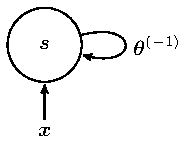
\includegraphics[]{figs/recurrent.pdf}
    \end{center}
    \caption{cyclic}
    \label{fig:recurrent}
  \end{subfigure}
  \begin{subfigure}[]{.79\textwidth}
    \begin{center}
    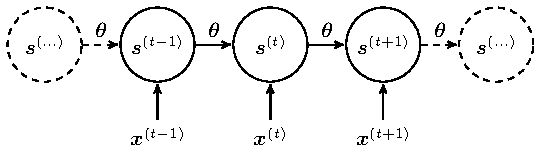
\includegraphics[]{figs/recurrent_uf.pdf}
    \end{center}
    \caption{acyclic (unfolded)}
    \label{fig:recurrent_uf}
  \end{subfigure}
  \caption{Recurrence Graph Views}
  \label{fig:recurrence}
\end{figure}


\section{Basic Recurrent Neural Network}

The functionality of a basic RNN resembles that of a traditional neural network with the addition of a state variable shared over time.


The core RNN functionality can be formulated as Equations \ref{eqn:rnn} describe. Each equation represents a `layer' or `node' in the network.
% no new para
\begin{subequations}  
  \label{eqn:rnn}
  \begin{align}
    \s\tm{t}&=
              \mathrm{\tanh}(
              \mt{W}_{ss}
              \s\tm{t-1}
              +
              \mt{W}_{xs}
              \x\tm{t}
              +
              \vc{b}_s
              ) 
              \label{eqn:rnns} \\ 
    \vc{o}\tm{t}&=
             \mt{W}_{so}
             \s\tm{t}
             +
             \vc{b}_{o}
             \label{eqn:rnno}
  \end{align}
\end{subequations}
\noindent 
The output at time $t$, $\vc{o}\tm{t}$, depends on current state, $\s\tm{t}$, which, in turn, depends on the previous state, $\s\tm{t-1}$, and the current input, $\x\tm{t}$, through associated weight matrices, $\mt{W}$. The weight matrices are subscripted with two variables to associate an input with an output. The input variable is the first subscript while the output variable is the second. For example, $\mt{W}_{so}$ connects the input from $\s$ to output, $\vc{o}$. Also, bias vectors, $\vc{b}$ allow values to be adjusted additively (offset). Finally, the hyperbolic tangent, $\tanh$, provides a non-linearity that allows the RNN to summarize arbitrarily complex sequences.

A `size' can be specified that measures the capacity of $\s$; the dimension of $\s$ is a (free) parameter (obviously the dimensions of other quantities in Equation \ref{eqn:rnns} need to be compatible).
%
No size is associated with $\vc{o}$ because it is restricted by the dimension of a given output, $\vc{y}$ (read further).

The output, $\vc{o}$, needs to be need to be compared to a `target', $\vc{y}$, through a loss function, $L$. For predicting sequences as targets, the mean squared error is a common choice for the loss function. Squared differences are summed and averaged over and the number of variables of the sequence resulting in a scalar as shown in Equation \ref{eqn:mse}.

\begin{equation}
  \label{eqn:mse}
  L(\vc{o},\vc{y}) = \frac{1}{TV} \sum_t \sum_v(
  \vc{o}\tm{t}_v - \vc{y}\tm{t}_v
  )^2,
\end{equation}
\noindent
$V$ and $T$ are the number of variables and the length of the sequences respectively indexed by $t$ and $v$ respectively.

Equations \ref{eqn:mse} and \ref{eqn:rnn}, together, define the framework for a basic RNN. One way to enhance this is to `stack' states so that the output from one state is input into another state in the same time step. So the last, $n$th, layer produces $\vc{o}$.  There is evidence that stacking the state layers leads to the network being able to learn time series at multiple time scales \cite{Hermans2013} \cite{Pascanu2013a}.

The stacking can be seen graphically in \ref{fig:rnn}.

\begin{figure}[H]
  \centering
  \begin{subfigure}[]{.2\textwidth}
    \begin{center}
    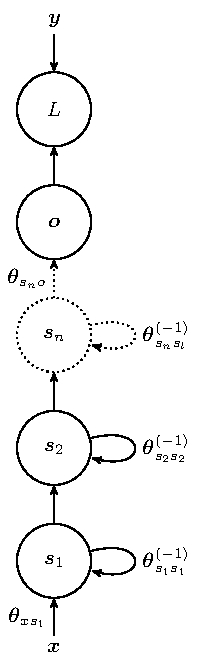
\includegraphics[]{figs/rnn.pdf}
    \end{center}
    \caption{cyclic}
    \label{fig:rnn_f}
  \end{subfigure}
  \begin{subfigure}[]{.79\textwidth}
    \begin{center}
    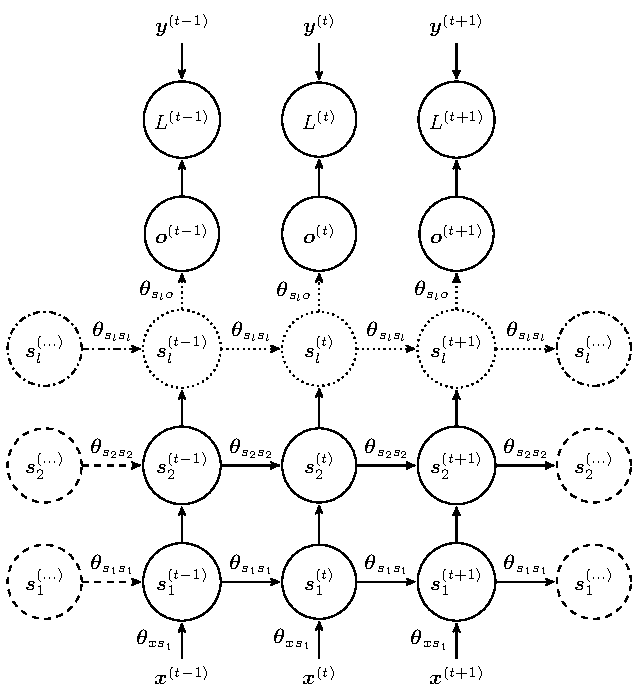
\includegraphics[]{figs/rnn_uf.pdf}
    \end{center}
    \caption{acyclic}
    \label{fig:rnn_uf}
  \end{subfigure}
  \caption{Recurrent Neural Network Graph Views}
  \label{fig:rnn}
\end{figure}
\noindent
%
Bias terms are omitted for clarity but are included as elements in $\vc{\theta}$ along with elements from $\W$.
%
The notation of $\vc{\theta}$ follows that of $\mt{W}$ but captures more variables by vectorizing each component for concatenation into a single vector.
%
$\vc{\theta}_{ss} = (\vc{W}_{ss},\vc{b}_s)$, $\vc{\theta}_{xs} = (\vc{W}_{xs})$, and $\vc{\theta}_{so} = (\vc{W}_{so},\vc{b}_o)$ (mathematical operations to produce the vector are implied).


Notice that the unfolded view allows one to see that information can flow through many paths in time and layers (horizontally and vertically respectively). So `depth' can be used to describe the number of operations in these two directions with depth in the time direction being typically much greater. This makes RNNs, among `deep learning' architectures, the deepest networks!


\section{Training}

%use s_(l)ayers. todo

To train the network, the loss function is used to  minimize (optimized) an objective function given pairs of training examples, $(\x,\vc{y})$, by adjusting the parameters $\vc{\theta}$. Unfortunately, training neural networks in general, let alone recurrent neural networks, are challenging optimization and computational problems \cite{Blum1992}. However, a flavor of the relatively simple mini-batch stochastic gradient descent (SGD) has remained successful in training a variety of networks \cite{Bengio2012b} despite the availability of other, perhaps more sophisticated, optimization algorithms. %practical recs for training deep. todo 2014+ ref?

In plain mini-batch SGD, parameters are updated with a `learning reate', $\alpha$, for a selected `mini-batch' example set (from the training set), $M$, according to Equation \ref{eqn:sgd} until a convergence critereon is met.

\begin{equation}
  \label{eqn:sgd}
   \Delta \vc{\theta} =
   -\alpha
   \frac{1}{|M|} \sum_{(\vc{x}_m,\vc{y}_m) \in M}
   \frac{\partial{L}(
     \vc{o}%(\x_m;\vc{\theta})
     ,\vc{y}_m)}
   {\partial{\vc{\theta}}}
\end{equation}
%todo: make  summation bigger

Unfortunately, RNNs can suffer acutely from the vanishing (and exploding) gradient problem which makes learning long range dependencies difficult \cite{Hochreiter,Bengio1994,Doya1992,Pascanu2013c}.

The problem is understood through the calculation of $\partial{L}/\partial{\vc{W}_{ss}}$ for a `history' of $T$ points prior to $t$.
%
An involved application of the (backpropagated) differential chain rule to the loss function using the \emph{basic} (unfolded) RNN defined in Equations \ref{eqn:rnn} leads to Equation \ref{eqn:grad}.

\begin{equation}
  \label{eqn:grad}
  \frac{\partial{L}\tm{t}}{\partial{\vc{W}_{ss}}} = 
  \sum_{i=0}^T
  \frac{\partial{    L}\tm{ t}}{\partial{\vc{o}\tm{t}}}
  \frac{\partial{\vc{o}}\tm{t}}{\partial{\vc{s}\tm{t}}}
  \left(
    \prod_{j=i+1}^{T}
    \frac{\partial{\vc{s}}\tm{j}}{\partial{\vc{s}\tm{j-1}}}
  \right)
  \frac{\partial{\vc{s}}\tm{i}}{\partial{\vc{W}_{ss}}}
\end{equation}
%
\noindent
Equation \ref{eqn:grad} shows that there are multiplicative `chains' of differentials for each preceding time step. 

The computational graph in Figure \ref{fig:grad}, represents Equation \ref{eqn:grad} for $T=4$.
%
\begin{figure}[H]
  \centering
  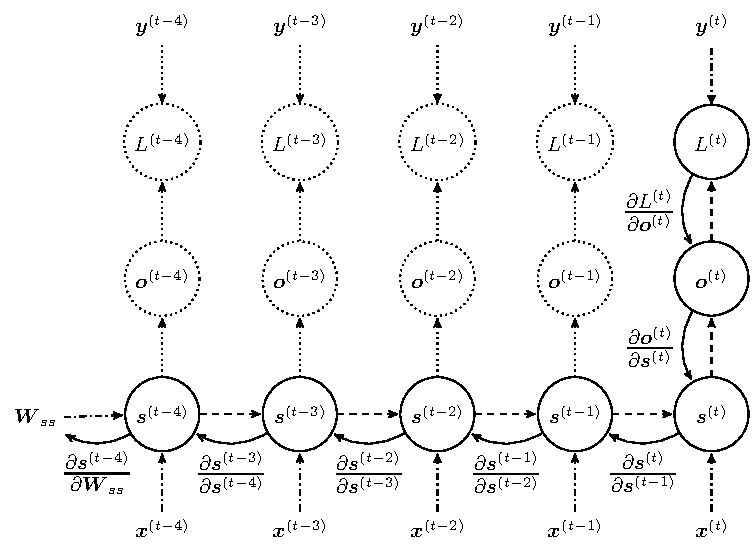
\includegraphics[]{figs/grad.pdf}
  \caption{Partial derivative chain for a basic RNN for a history of 4 time steps (biases not shown)}
  \label{fig:grad}
\end{figure}
%
\noindent
Several quantities are distinguished. Dash-dotted lines are the independent inputs, $\x$, $\vc{y}$, and $\vc{W}_{ss}$, to the loss function, $L$, while the dashed lines represent intermediate quantities in the graph.
%
The path formed by the curved solid lines follows the chain rule to get one summand for $\partial{L}\tm{t}/\partial{\vc{W}_{ss}}$.
%
Dotted quantities are not involved in the calculation (for $T=4$).


Now that the graph is associated with the equation, the origin of the vanishing granient can be seen;
%
the vanishing gradient is due to successive multiplications of the derivative of $\tanh$ which is bound in $(0,1]$ (Again, see \cite{Hochreiter,Bengio1994,Doya1992,Pascanu2013c} for details).


\cite{Bengio-et-al-2015-Book} (sec. 10.7) lists ways in which the problem can be mitigated by applying different RNN architectures or enhancing the optimization process.
%
For example, Hessian-free optimization \cite{Martens2010} uses second order information that can make use of the ratio of small gradients to small curvature to more directly find optimal parameters.
%
\cite{Martens2011} uses Hessian-free optimization to train (a basic) RNN to achieve remarkable results.
%
However, this comes at a computational cost.
%
For practical reasons, it might be preferrable to use well-established SGD-based methods over second order methods \cite{Bengio2012,Dauphin} as long as the RNN architecture facilitates learning long range dependencies;
%
the Long Short Term Memory (LSTM) RNN \cite{Hochreiter1997} uses a `memory cell' to recall (past) information only when needed thereby working around the vanishing gradient problem.




\section{Long Short-Term Memory} %todo check hyphenations

LSTM models have acheived impressive benchmarks recently.
%
Networks with LSTM elements have been used for
text-to-speech synthesis \cite{Fan2014},
language identification from speech \cite{Gonzalez-Dominguez2014},
large-vocabulary speech recognition \cite{Sak2014},
English-to-French text translation  \cite{Sutskever2014},
identifying non-verbal cues from speech \cite{Brueckner2014},
Arabic handwriting recongition \cite{Bluche},
image caption generation \cite{Vinyals2015},
video to text description \cite{Venugopalan2014},
and generating realistic talking heads \cite{Fan2015}.
%
Futhermore, LSTM RNNs have remained competitive against other RNN types \cite{Jozefowicz2015}.


There are a few variants of LSTM but they all have a linear self-loop that gradients can flow through for a long time.
%
LSTM variants have not shown to differ greatly in performance \cite{Greff2015}.
%
The equations describing the LSTM state involve significantly more steps than the basic RNN state equation, Equation \ref{eqn:rnn}.
%
So, the mathematical procedure for the LSTM state is presented with a figure.
%
The LSTM variant presented in Figure \ref{fig:lstmfig} is found in \cite{Graves2013b}.

\begin{figure}[H]
  \centering
  \begin{subfigure}[]{\textwidth}
    \begin{center}
    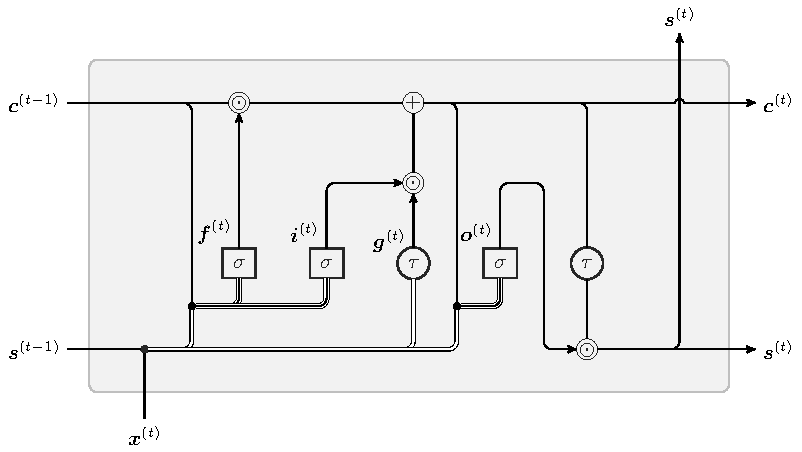
\includegraphics[]{figs/lstm.pdf}
    \end{center}
    \caption{calculation flow diagram (biases omitted, inspired by \cite{Colah2015})}
    \label{fig:lstm} 
  \end{subfigure}
  \begin{subfigure}[]{\textwidth}
    \begin{subequations}
      \begin{align}
        \vc{i}\tm{t} 
        &= 
          \sigma
          (
          \mt{W}_i \cdot
          (
          \x\tm{t},
          \vc{h}\tm{t-1},
          \vc{c}\tm{t-1}
          )
          +\vc{b}_i
          ) 
        \\
        \vc{f}\tm{t} 
        &=
          \sigma
          (
          \mt{W}_f \cdot
          (
          \x\tm{t},
          \vc{h}\tm{t-1},
          \vc{c}\tm{t-1}
          )
          +\vc{b}_f
          )
        \\
        \vc{g}\tm{t}
        &=
          \tanh
          (
          \mt{W}_c \cdot
          (
          \x\tm{t},
          \vc{h}\tm{t-1}
          )
          +\vc{b}_c
          )
        \\
        \vc{c}\tm{t} 
        &= 
          \vc{f}\tm{t}   \odot \vc{c}\tm{t-1}
          + \vc{i}\tm{t} \odot \vc{g}\tm{t}
        \label{eqn:lstms}\\
        \vc{o}\tm{t}
        &=
          \sigma
          (
          \mt{W}_o \cdot
          (
          \x\tm{t},
          \vc{h}\tm{t-1},
          \vc{c}\tm{t-1}
          )
          +\vc{b}_o
          )
        \\
        \vc{h}\tm{t}
        &=
          \vc{o}\tm{t} \odot
          \tanh
          (
          \vc{c}\tm{t}
          )
      \end{align}
    \end{subequations}
    \caption{equations}
    \label{eqn:lstm}
  \end{subfigure}
  \caption{Long Short-Term Memory Module}
  \label{fig:lstmfig}
\end{figure}
\noindent
%
$\sigma$ stands for the logistic sigmoid function while $\tau$ stands for $\tanh$.
%
Elementwise multiplication is represented by the $\odot$ symbol.
%
For brevity and clarity, a (single) weight matrix combines the weights associated with more than one input to a single output (unlike the typical notation used in literature).
%
For example, $\mt{W}_i \cdot(\x\tm{t},\vc{h}\tm{t-1},\vc{c}\tm{t-1})=\mt{W}_{xi}\vc{x}\tm{t}+\mt{W}_{hi}\vc{h}\tm{t-1}+\mt{W}_{ci}\vc{c}\tm{t-1}$ where the input vectors, $\x$, $\vc{h}$, and $\vc{c}$ are concatenated into a vector  and weight matrices $\mt{W}_{xi}$, $\mt{W}_{hi}$, and $\mt{W}_{ci}$ are augmented horizontally. %todo.. chk dim in theanets code
%
In the diagram, the concatenation is represented by black dots combining single lines into more than one line.
%
Furthermore, $\mt{W}_{ci}$, $\mt{W}_{cf}$, and $\mt{W}_{co}$ are diagonal matrices so the number of weights associated with each $\vc{c}$ equals the LSTM `size'.


The size that can be attributed to the LSTM module is the dimension of $\vc{i}$, $\vc{f}$, $\vc{c}$, $\vc{g}$, $\vc{o}$, or $\vc{h}$ which are equal.


Very briefly, the central element in a LSTM module is the `memory cell', $\vc{c}$, that works to keep information unchanged over many time steps (likened to a conveyor belt through time).
%
Information flow is controlled through input, forget, and output `gates', elements $\vc{i}$, $\vc{f}$, and $\vc{o}$ respectively.
%
The input gate controls information into the memory cell.
%
The output gate controls when information should flow to the next time step.
%
The forget gate zeros out elements in the memory cell.
%
The gates make their decisions based on the input, $\x$, the `hidden' state, $\vc{h}$, and content already in the memory cell.
%
%g is a c candidate
%things get trapped in memory

%c has stuff nominally 0-1 while h has -1,1 behaves more like regular rnn
% how c 0,1 if g can be -1,1
% i can imagine if c had a 1. there would be a way for it to stay
%things could be simpler in alt. to LSTMS!
%original lstm paper to know whys of everything

% The following enumeration conceptually outlines the operation of the LSTM module.

% \begin{enumerate}
% \item[1. ] sfd
% \end{enumerate}

% proc
% 1
% 2
% 3

% math that shows lstm gets around vanishing grad

Unlike the recurrence of the basic RNN (Equation \ref{eqn:rnns}), information can be kept for a long time in the recurrence chain of $\vc{c}$ (Equation \ref{eqn:lstms}). 
%
There is a way for information to propagate without successive multiplication of fractions (as in the derivative of $\tanh$):
%
Consider an element in (vector) $\vc{c}\tm{t-1}$ with a value of 1.
%
It can be retained indefinitely as long as the corresponding element in $\vc{f}\tm{t}$ is 1 and the corresponding element in $\vc{i}\tm{t}$ is 0.
%
In other words, the derivative is constant.

Finally, note how the LSTM modules can be stacked (vertically) in similar fashion to the basic RNN.
%
The output of the lower module, $\vc{h}\tm{t}$, becomes the input, $\x\tm{t}$, of the upper module.


With such configurations, the next chapter will show how LSTM RNNs can be used to model time series to find anomalies.

% lstm:
% CECs are
% the main reason why LSTM nets can learn to discover the importance of (and memorize) events that
% happened thousands of discrete time steps ago, while previous RNNs already failed in case of minimal
% time lags of 10 steps


%%% Local Variables:
%%% mode: latex
%%% TeX-master: "thesis"
%%% End:

\chapter[]{Anomaly Detection Using Recurrent Neural Networks}


\section{Introduction}

Chapters \ref{ch:ad} and \ref{ch:rnn}, separately, introduced anomaly detection in time series and recurrent neural networks as time series modelers.
%
This chapter outlines a procedure for finding anomalies using RNNs with the goal of mitigating many of the problems associated with anomaly detection that were discussed in \ref{ch:ad}.
%
As much as possible, the same procedure is applied to some time series.


The outlines describes:
%
\begin{description}
%
\item[sampling:] the time series used for training and its associated sampling process
%
\item[recurrent autoencoders:] the specific form of the RNN
%
\item[training:] the training algorithm used on the RNN
%
\item[Bayesian optimization:] the search for optimized parameters for the procedure
%
\end{description}



\section{Sampling}


Some time series with anomalies were chosen or generated to test the anomaly detection process.
%
While there is only one `master' time series to train on (in each test), the RNN needs to see many `samples' from the master time series.
%
The sliding window procedure, described in \ref{sec:adsample}, is used to get samples of some window length.
%
Additionally, since RNNs do not need a fixed window, sliding windows are obtained for more than one window length.
%
Furthermore, the samples are organized into `mini-batches' (of the same window length) to be more compatible with the training procedure.
%
The window length is incremented (size skip) from some minimum until it is not possible to obtain a mini-batch (so the largest window will be close to the length of the time series).


Table \ref{tbl:winspec} specifies the relevent sizes and increments for the sampling process.
%
The values were adjusted manually until a `reasonable' number of samples were found.
%
However, the minimum window length was chosen such that meaningful dynamics were captured (regardless of the scale of the anomaly).

\begin{table}[H]
\centering
\begin{tabular}{|l||c|c|c|c|c||c|}
  \hline
  series & length & min. win. & slide skip & size skip & batch size & $\Rightarrow$ num. samples
  \\ \hline \hline
  sine (gen.) & 1000 & 100 & 10 & 10 & 30 & 96 
  \\ \hline
  ecg \cite{PhysioNet} & 3277 & 300 & 20 & 20 & 30 & 300
  \\ \hline
  spike (gen.) & 800 & 80 & 8 & 8 & 10 & 378
  \\ \hline
  power \cite{Keogh2005} & 7008 & 100 & 100 & 20 & 30 & 121
  \\ \hline
  sleep \cite{this} & 2560 & 300 & 20 & 20 & 30 & 165
  \\ \hline
\end{tabular}
\caption[]{Time series sample specifications} %todo: what case?
\label{tbl:winspec}
\end{table}



   % ts=get_series(id)
   %  tnth=int(.1*len(ts))
   %  kwargs.setdefault('min_winsize',        int(    tnth))
   %  kwargs.setdefault('slide_jump' ,        int(.10*tnth))
   %  kwargs.setdefault('winsize_jump',       int(.10*tnth))
   %  kwargs.setdefault('batch_size',         10           )
    
   %  if 'ecg'==id:
   %      kwargs['min_winsize']=  300
   %      kwargs['slide_jump']=   20
   %      kwargs['winsize_jump']= 20
   %      kwargs['batch_size']=   30

   %  elif 'sleep'==id:
   %      kwargs['min_winsize']=  300
   %      kwargs['slide_jump']=   20
   %      kwargs['winsize_jump']= 20
   %      kwargs['batch_size']=   30

   %  elif 'sin'==id:
   %      kwargs['batch_size']=   30

   %  elif 'twitter'==id:
   %      kwargs['batch_size']=   30
   %      kwargs['min_winsize']=  4000

   %  elif 'power'==id:
   %      kwargs['min_winsize']=  1000
   %      kwargs['slide_jump']=   500
   %      kwargs['winsize_jump']= 200
   %      kwargs['batch_size']=   30









\section{Training}

for detailed overall trning: 'How large should the batch size be for stochastic gradient descent?'


'advances in optimizing recurrent nn' enhanced sgd still competitive or better
'Equilibrated adaptive learning rates for non-convex optimization' -rmsprop is good. sgd good but issue is just how to adjust weights.


%%% Local Variables:
%%% mode: latex
%%% TeX-master: "thesis"
%%% End:

\chapter{Concluding Remarks}
%todo. rename everything to sequence. seq. includes ts

Now that proximity-based and model-based anomaly detection techniques have been introduced in Chapter \ref{ch:ad}, some comparisons can be made with them given the results from the previous chapter.
%
From there, some qualified conclusions can be made.
%
Mind that, from the start, the comparison is made with techniques that do not require labeled data.
%
Also, the comparison is made as general statements of advantages of RNNs over the alternative.

\begin{description}


\item Hidden Markov Models (model).

      Chapter \ref{ch:rnn}, explained how, fundamentally, RNNs store states more efficiently.
      %
      By itself, this does not provide a functional advantage over HMMs, but this requires an HMM for every sequence length, unlike RNNs.
      %
      Furthermore, while HMMs are powerful, RNNs are fundamentally sequence modelers.


\item HOT SAX (proximity).

      The HOT SAX \cite{Keogh2005} technique (and its variants) is considered a proximity-based technique optimized for sequences that is sensitive to window size.
      %
      While the results show in the previous chapter that window size is important, RNNs have the advantage that, the same RNN can be used to find anomalies at different scales.
      %
      In HOT SAX, a comparison is made for almost all pairs of windows for one window size.
      %
      This thorough comparison may be tolerable for short sequences, but a \emph{trained} RNN can analyze a long sequence for anomalies based on a shorter sample.
      %
      Furthermore, the mathematics of RNNs naturally accept multivariate sequences.


\end{description}


Through the previous discussion, the advantage of using autoencoding RNNs as described in this work, in comparison to other techniques, can be summarized in a few questions.
%
A negative response to the following questions for the alternative gives RNNs an advantage.

\begin{itemize}

\item Is only the test sequence needed to determine how anomalous it is?%
\footnote{This is related to generative versus discriminative models. Generative models are preferred for anomaly detection.}
(Is a summary of the data stored?)

\item Is it robust against some window length?

\item Is it invariant to translation? (Is it invariant to sliding a window?)

\item Is it fundamentally a sequence modeler?

\item Can it handle multivariate sequences?

\item Can the model prediction be associated with a probability \cite{Graves2013b}?

\item Can it work with unlabeled data? If not, is it robust to anomalous training data?

\item Does it require domain knowledge?

\end{itemize}


Finding a technique with all these advantages is difficult.
%
But, as mentioned in the Introduction chapter, the work in \cite{Malhotra2015} is the closest to the work described here so some comparison is merited.
%
In \cite{Malhotra2015}, the RNN is trained to predict a set length of values ahead for every (varying length) subsequence that starts at the first point%
\footnote{Clarification provided in electronic exchange with author, P. Malhotra.}% obvioiusly you need this pct sign here!
.
%
Although this training setup was used to avoid dealing with windows (as an advantage), the choice of the prediction length remains arbitrary and its effect on finding anomalies at different scales is not studied.
%
In this work, although windows were found to be needed to detect anomalies, the only choice made regarding their length was to set some minimum meaningful length for the training samples%
\footnote{Another way of seeing the difference in the mode of operation between the two RNN setups is by considering their mappings. In \cite{Malhotra2015}, an arbitrary subsequence is mapped to a fixed length sequence while in this work an arbitrary subsequence is mapped to itself.}
(not the scale of the anomaly).
%
In fact, specifying a window size for the prediction errors (as in Section \ref{sec:results}) can be seen as an advantage because it allows detection of anomalies at different scales as a desired choice for the investigator.
%
Furthermore, \cite{Malhotra2015} uses normal data for training thereby not providing evidence that their process can tolerate anomalous data.
%
But in contrast to this work, evidence for anomaly detection in multivariate time series is provided.
%so each pt has all previous predeicted length times
%they used a set prediction output seq. unlike AE.
%they also do not prove that it works by using ALL data
%but they show multivar unlike here
%how far out makes sense?
%diff pred strenghts for a pt and surely rnn can't predict that far ahead

Unfortunately, the power of RNNs comes at high computational expense in the training process.
%
Not only is there a cost in finding RNN parameters ($\vc{\theta}$), but there is also a cost in finding RNN hyper-parameters which can include parameters specifying RNN architecture as well as parameters specifying training algorithm parameters.


Given the results of this work and how it compares to other techniques, it can be concluded that autoencoding RNNs can be used to detect anomalies in arbitrary sequences, provided that an initial training cost can be managed.


\section{Further Work}

The text ends with a list of further work directions with potential to strengthen the case for using autoencoding RNNs in anomaly detection.
%
As the list is mainly concerned with the RNNs, and much progress has been made in RNN research recently, the list is not exhaustive.
%
Furthermore the rapid progress might render items in the list as outdated in the near future.


\begin{description}[style=unboxed]


\item[Better optimize presented work.]

More training epochs and more LSTM layers could have found more optimized parameters.
%
Also, variations in the training data on the length scale of the sequence (trends) should be removed.
%
These optimizations are important to effectively learn normal sequence patterns.


\item[Use autocorrelation to determine a minimum window width.]

In the sampling process, the minimum window length was manually determined such that the length captured meaningful dynamics.
%
This length can be systematically determined by using information from the sequence's autocorrelation.


\item[Accelerate training.]  \hfill %obviously no need for \\ obviously

                 \begin{description}


                 \item[Normalize input.]

                 Although not required, some carefully chosen normalization of data could help.
                 %
                 Another normalization scheme to consider is found in a a recent paper \cite{laurent2015batch} which suggests using normalization based on mini-batch statistics to accelerate RNN training.
                 

                 \item[Find an optimum mini-batch size.]
                 
                 Some redundancy in the mini-batch is desired to make smooth progress in training.
                 %               
                 However, if the mini-batch size is too large (too redundant), a gradient update would involve more computations than necessary.
                          
                 \end{description}

\item[Use dropout to guard against overfitting.]
%
In this work, to guard against overfitting, a corrupting signal is added which depends on the value of the data.
%
In dropout, regardless of the values of the data, a small portion of nodes in a layer can be deactivated allowing other nodes to compensate.
%
Dropout was first applied to non-recurrent neural networks but recent study \cite{Zaremba2014} explains how dropout can be applied to RNNs.


\item[Experiment with different RNN architectures.] \hfill


                 \begin{description}[style=unboxed]%yeaa just this one but not others!!!


                 \item[Experiment with alternatives to the LSTM layer.]

                 Over a basic RNN, the LSTM imposes more computational complexity as well as more storage requirements (for the memory cell).
                 %
                 Gated Recurrent Units (GRU) \cite{Cho2014} are gaining in popularity as a simpler and cheaper alternative to LSTM layers.


                 \item[Experiment with bi-directional RNNs.]

                 Bi-directional RNNs \cite{Schuster1997} incorporate information in the forward as well as reverse direction.
                 %
                 They have been successfully used with LSTM for phoneme classification \cite{Graves2005}.


                 \item[Experiment with more connections between RNN layers.]

                 A better model might be learned if the layers are connected \cite{Hermans2013} (through weights) because it allows for more paths for information to flow through.

                 \end{description}


\item[Incorporate uncertainty in reconstruction error.]

Thee output from a RNN can be interpreted to have an associated uncertainty \cite{Graves2013b}.
%
It follows that it should be possible to get high or low error signals associated with high uncertainty which should affect the interpretation of the existence of an anomaly (see Reconstruction Distribution, Section 13.3, in \cite{Bengio-et-al-2015-Book}).


\item[Objectively compare anomaly detection performance against other techniques
 over a range of data.] 


While certain disciplines might have benchmark datasets to test anomaly detection, measuring the generality of a technique by evaluating its performance over a wide variety of data is not widespread%
\footnote{Perhaps this is due to the difficulty in finding a general technique.}%
.
%
To solve this problem, Yahoo recently offered a benchmark (labeled) dataset \cite{Laptev2015} which includes a variety of synthetic and real time series.


Methods based on non-linear dimensionality reduction might be competitive \cite{Lewandowski2010}.


\item[Find anomalies in multivariate sequences.]

The NASA Shuttle Valve Data \cite{Ferrel2005} is an example which was used in \cite{Jones2014} and the well-known HOT SAX \cite{Keogh2005} technique.


%questions: why pt errs not reveal anoms?? but this does not further my goal
% what relation b/w stats anom and ML

\end{description}




%todo: fix margin on nested descriptions

%%% Local Variables:
%%% mode: latex
%%% TeX-command-extra-options: "-shell-escape"
%%% TeX-master: "thesis"
%%% End:
%%
%%  bibliography

%% list all of the BibTeX files here for the WinEdt project (if applicable)
%GATHER{bibfile.bib}

%% any bibliography style can be used, but IEEEtran.bst is ideally suited to
%% electrical engineering references





%% include the following directives if there are any appendices
\appendix
\appendixeqnumbering
%% A sample appendix
%%
%%**********************************************************************
%% Legal Notice:
%% This code is offered as-is without any warranty either
%% expressed or implied; without even the implied warranty of
%% MERCHANTABILITY or FITNESS FOR A PARTICULAR PURPOSE!
%% User assumes all risk.
%% In no event shall any contributor to this code be liable for any damages
%% or losses, including, but not limited to, incidental, consequential, or
%% any other damages, resulting from the use or misuse of any information
%% contained here.
%k%**********************************************************************
%%
%% $Id: Appendix.tex,v 1.6 2006/08/25 00:58:50 Owner Exp $
%%

% N.B.: an appendix chapter starts with "appchapter" instead of "chapter"
%
% The first argument in [ ] is the title as displayed in the table of contents
% The second argument is the title as displayed here.  Use \\ as appropriate in
%   this title to get desired line breaks
%\appchapter[An Appendix]{An Appendix}


\chapter{Reproducible Computational Infrastructure}


\section{Introduction}


There has been much attention recently on being able to reproduce computational research \cite{Stodden2013}. 
%
In some cases, just providing the computational code and data, along with some instructions, is sufficient to be able to reproduce a computational experiment.
%
However, typically code relies on libraries and other support facilities which complicates the computational setup.
%
So, just providing the computational code is not sufficient to ensure reproducibility (at least not easily).
%
Some domains have managed this complexity somewhat by providing specific solutions.
%
As examples, \textsf{Galaxy} is used in genome analysis \cite{Giardine2005},
%
\textsf{Madagascar} in geophysics \cite{Fomel2013},
%
\textsf{WaveLab} in signal processing \cite{Buckheit1995},
%
and \textsf{Bioconductor} in computational biology and bioinformatics \cite{Gentleman2004}.
%
These solutions can be seen as platforms onto which instructions can be provided.


However, these solutions do not address computational infrastructure setup in addition to being limited to their domains.
%
`Infrastructure' here means aspects related to both hardware and software.
%
While the importance of hardware is not emphasized as much as software in reproducibility%
\footnote{This is because the quantitative programmer is usually highly removed from hardware details. The same cannot be said of software dependencies.}%
,
it is best to think of hardware as clean slates onto which software is installed, beginning with the operating system.
%
In fact, some computational code requires certain hardware like graphics processing units (GPUs).
%
Furthermore, computational codes might interact with (non-computational) services provided by the operating system and/or non-computational services that perhaps are closely associated with the operating system.
%
Therefore providing instructions, in the form of code, that specify the hardware \emph{and} software has much value for reproducibility.
%
The benefit from having such instructions is not limited to ensuring integrity of results;
%
the iterative work process is greatly enhanced because this level of reproducibility implies automation.


Many software tools from information technology (not specific to high-performance computing) automate infrastructure setup.
%
As such, the results presented in Chapter \ref{ch:results}, were obtained by using an automated process that used some of these information technology tools.
%
Futheremore, while being motivated by a problem encountered in this work, the process has been separated out as an independent solution applicable to any computational problem.


The following sections describe the problem and, in turn, its solution.


\subsection{Motivation}

The Bayesian optimization process, explained in Section \ref{sec:training}, required the coordination of many components.
%
The general problem is explained here but refer to Chapter \ref{ch:reproduce} for the specific solution components.
%
The components must satisfy the following requirements:
%
\begin{itemize}

\item 
  the provisioning of a \textsf{mongodb} database so that \textsf{spearmint} could store its optimization progress in it

\item
  the provisioning of a database to store RNN parameters after every training iteration

\item
  the coordination of training runs on potentially multiple compute machines where a RNN training run is for certain hyper-parameters (a course form of parallelization)

\end{itemize}

Furthermore, two operational requirements can be added as well:

\begin{itemize}

\item
  There should be an automated (reproducible) process that sets up these components.

\item
  The investigator should be able to seamlessly transition from testing and development on his/her local machine to `production' execution on a remote machine.
%
That is, the investigator's workflow should be uninterrupted.

\end{itemize}


So the challenge is twofold: the reproducibility of each component and the reproducibility of the setup.
%
Also, this implies that the setup should occur in clean, isolated environments.


\section{Solution Elements}


Some solutions solve certain parts of the previously listed requirements.
%
They ccan be evaluatd based on their degree of reproducibility and automation.


\begin{description}


\item[local virtual machine: \textsf{VirtualBox}.]
  %
  This software virtualizes all the workings of a machine into a process running on a (local) host operating system.

  
  However, on its own, \textsf{VirtualBox} does not provide a systematic and generic way of provisioning the machine as well as provisioning software on the machine.


\item[local virtual machine automation: \textsf{Vagrant}.]
  %
  By providing \textsf{Vagrant} with instructions in a file, virtual machine setup can be automated.
  

  \textsf{Vagrant} can control \textsf{VirtualBox} by specifying virtual machine hardware as well a machine image (file) which typically includes an operating system installation at least.
  %
  While a virtual machine provisioned automatically provides an isolated, reproducible environment for work, it needs to exist in the context of being a part of a network of machines.
  %
  So, ideally, after a minimal initial provisioning, the virtual machine is treated as just another machine regardless of the fact that it exists virtualized locally.


\item[application reproducibility: \textsf{Docker}.]
  %
  From instructions in a file, \textsf{Docker} can create an isolated application image.


  \textsf{Docker} has recently emerged as an easy yet powerful way to work with (isolated) application containers.
  %
  Furthermore, the image execution is portable as long as the machine has compatible architecture which has obvious advantages when working with multiple machines.
  %
  Also, by persisting the image, the application can be started swiftly since the image creation process would have already gone through potentially lengthy software installation processes.
  %
%footnote? docker like vm but compare to handling vm img!
  %
%used for svc and the compute code as well.
%
  In the context of computational research, it is possible to have isolated, reproducible containers for, as examples, databases, computational code, and computational task management.
  %
  While \textsf{Docker} provides a great deal of reproducibility, it is not involved in machine provisioning.



\item[distributed \textsf{Docker} support: \textsf{Weave} and \textsf{CoreOS}.]
%
\textsf{Weave} and \textsf{CoreOS} facilitate the distributed operation of \textsf{Docker} containers.

Given that \textsf{Docker} was identified as an important solution component, it follows that \textsf{Docker}-specific solutions should be chosen that facilitate distributed application execution.
%
\textsf{Weave} provides global private network addressing for each container.
%
\textsf{CoreOS} a \textsf{Linux} operating system designed for distributed, containerized applications.
%
As such, it is delivered with mimimal software and services as containers are assumed to be the primary method by which software and services are added.
%
In the context of computational research, this ensures the fastest possible execution of computational code since the operating system is not running unnecessary processes.
%docker soles other probs but these are main ones

\item[remote machine facility: \textsf{Amazon Web Services (AWS)}.] 
  %
  \textsf{AWS} provides high-performance compute machines, including machines equipped with GPUs, running \textsf{CoreOS}.
  

  What is important for the purpose of automation, is that \textsf{AWS} provides a programmatic interface for the provisioning of machines.
  % 
  However, the choice of \textsf{AWS} is not critical because \textsf{AWS} can be substitued by other providers providing comparable facilities.
 


\item[global automation: \textsf{Ansible}.]
  %
  \textsf{Ansible} is the highest-level automation software that can orchestrate the infrastructure setup process (in full).
  
  \textsf{Ansible} can be used to generically provision machines, local or remote, virtual or physical.
  %
  \textsf{Ansible} can also be used to provision software, containerized or not.
  %
  Furthermore, the provisioning of hardware and software can occur in a coordianted fashion.


\end{description}


\subsection{Solution Stack}
\label{sec:stack}


The solution elements can be organized into a `stack' to help understand their place in an overall solution.
%
The stack represents a technology dependency which is depicted in Figure \ref{fig:stack}.
%
The goal is to be able to automatically recreate this technology stack anywhere.
%
As such, \textsf{Ansible} is not shown because it is an automation tool that sets up the stack.


\begin{figure}[h]
\newcolumntype{T}{!{\vrule width 3\arrayrulewidth}}
\newcolumntype{C}[0]{>{\centering\let\newline\\\arraybackslash\hspace{0pt}}m{1.5in}}
\centering
\begin{tabular}{l C C}
  \Xhline{6\arrayrulewidth}
  application   
  &  \multicolumn{1}{TcT}{\ldots}
  & \multicolumn{1}{TcT}{\ldots} 
  \\
  \hline
  container network 
  & \multicolumn{2}{TcT}{\textsf{Weave}}  
  \\
  app. containerization  
  & \multicolumn{2}{TcT}{\textsf{Docker}}   
  \\
  \hline
  operating system 
  & \multicolumn{2}{TcT}{\textsf{CoreOS}} 
  \\ 
  \hline
  machine 
  & \multicolumn{1}{TcT}{(x64)}
  &  \multicolumn{1}{TcT}{x64} 
  \\ 
  \hline
  hypervisor 
  & \multicolumn{1}{TcT}{\textsf{VirtualBox}} 
  & \multicolumn{1}{TcT}{\ldots }
  \\
  hypervisor interface
  & \multicolumn{1}{TcT}{\textsf{Vagrant}} 
  & \multicolumn{1}{TcT}{\textsf{AWS}}
  \\
  \hline
  host operating sys. 
  & \multicolumn{1}{|c|}{
    \textsf{Windows}%
    \textbar \textsf{OS X}%
    \textbar \textsf{Linux}
    }
  & \multicolumn{1}{TcT}{\ldots}
  \\
  \hline
  hardware 
  & \multicolumn{1}{|c|}{x64}
  & \multicolumn{1}{TcT}{x64}
  \\
  \Xhline{6\arrayrulewidth}
  & local 
  & remote
\end{tabular}
\caption[Container-oriented computational technology stack]
{Container-oriented computational technology stack.
%
Technologies bordered by thick lines are under the influence of automation by \textsf{Ansible}.
%
The parentheses around x64 indicate that the hardware architecture is virtualized (under type-2 hypervisor).
%
Table cells with ellipses are immaterial to the discussion.
%
}
\label{fig:stack}
\end{figure}


The reproducibility of results from computation (at the application layer) is generally not influenced by technologies lower in the stack.
%
In fact, they can be swapped with other technologies as long as the technology stack is compatible.


For reproduciblity of results, it is more a matter of convenience that the layers above the hypervisor can be recreated locally and remotely.
%
However, the technologies selected facilitate portability in several ways which allows for easier collaboration and reproducibility of results starting at different levels.
%
At the lowest level, the automation code can recreate the full stack, locally and remotely, perhaps with different hypervisors.
%
So, at the container level, \textsf{Docker} instructions can be used to recreate the application image.
%
Alternatively, the image (itself) can be transferred to any compatible machine for execution.
%
At the application level, only the most independent codes are truly portable.
%
Practically all modern computational codes have complex dependencies which are handled in a variety of ways.
%
But by using \textsf{Docker}, dependencies are handled in the most general way.


In fact, the level of encapsulation that \textsf{Docker} offers has  been compared to that of virtual machines (inaccurately%
\footnote{It is best to think of \textsf{Docker} containers as encapsulated \emph{processes}.}%
).
%
But unlike a virtual machine, it does not suffer from the additional overhead incurred by running an operating system and possibly virtualizing hardware as well.
%
In fact, the overhead of running \textsf{Docker} is negligible.
%
So if the concern is just running a typical application, transferring a \textsf{Docker} image is preferrable to transferring a virtual machine image%
\footnote{
Applications requiring specialized hardware such as GPUs are not as transferrable.
}%
.


But speaking of a `stack' on a machine, individually, does not address distributed computing.
%
Using multiple machines to accelerate computing is highly-desirable, if not essential, depending on the application.
%todo: is this sentence redundant?
%
This is where automating the entire stack on any compute provider, homogeneously, becomes advantageous since the automation code embodies the distributed environment.
%
Therefore, even the distributed environment can be reproducible.



\subsection{Partial Solutions}


Research-oriented cluster computing faciilties were found to not satisfy the requirements previously mentioned.
%
Typically, the machines are provided with an operating system installed with a restricted user account.
%
This restricts the ease in which some software can be installed although this can be mitigated somewhat if \textsf{Docker} is installed.
%
Most importantly, is that the use of research-oriented clusters does not facilitate a seamless transition from local development to remote execution because the local and remote environments do not match (unless the local environment is restricted to use the same technologies as the facility which would limit portability of the setup process).
%
So treating cluster computing providers as just providers of machines is advantageous because it allows the investigator generically automate the setup of the same computing environment on any facility.


While automating the setup for a research-oriented cluster is possible, \textsf{StarCluster} is notable for automating the setup for \textsf{AWS}.
%
Although the setup is convenient, \textsf{StarCluster} otherwise is much like a research-oriented cluster computing facility but with more control given to the user since adminitrative priviledges on the operating systems are granted.
%
Not only is \textsf{StarCluster} restricted to \textsf{AWS}, but its technology stack is not designed for the primary usage of \textsf{Docker}.
%
Furthermore, the argument holds that \textsf{StarCluster} does not facilitate the seamless transition from local development to remote execution due to the mismatch between the environments.



\section{Solution}


Section \ref{sec:stack} discussed the advantages of having a homogeneous computing stack on any hardware based on \textsf{Docker} solutions.
%
This section will exhibit a `base' infrastructure onto which complex distributed applications can run.
%
Figure \ref{fig:pcc} depicts the base infrastructure in a technology layer-oriented view.
%layer view. not net view.


\begin{sidewaysfigure}[h]

  \includegraphics[width=\textwidth]{appendix/figs/arch.pdf}

\caption[Generic infrastructure for distributed computation based on \textsf{Docker}]{
Generic infrastructure for distributed computation based on \textsf{Docker}.
%
Dashed boxes group networks.
%
The (dotted) \textsf{Weave} network crosses network boundaries.
}
\label{fig:pcc}
\end{sidewaysfigure}


The base infrastructure begins with setting up resources on a user's local machine to enable the execution of applications on remote machines.
%
Central to this is sharing local files which provides persistence of data and executables between instantiations of machines.
%




%mismatch


% use ansible to coordinate this. other coordiantion tools exist but ansible is a good base generic. lot's of support. customized for this workflow.


% major services of init: registry and storage

% benefits:
% code -> binary -> vm binary

% - last thing: usage instructions as in repo. this doc jsut high level more specifics in repo. and since details will change.

% adv:
% - code is portable b/c it is agnostic to compute facility
% - reproducible
% - worst case is running locally. guaranteed to work.


%%% Local Variables:
%%% mode: latex
%%% TeX-master: "../thesis"
%%% End:

\chapter{Reproducing Results}
\label{ch:reproduce}



\section{Introduction}


This chapter shows the commands that were issued to obtain the results shown in Chapter \ref{ch:results}.
% 
The commands build on the infrastructure setup explained in Chapter \ref{ch:pcc}.
% 
Also, the commands (themselves) specifically address requirements of the Bayesian optimization process driven by \textsf{Spearmint} as described in Section \ref{sec:pccmotivation}.
% 
As such they are the highest-level commands that can be automated as well but were not to give the investigator some control over execution.
% 
But the control is only operational as similar results should be obtained regardless of how the computations are executed.


However, first, a set of `manual' instructions are provided as well that are more typical of instructions accompanying computational publications (if at all!).
% 
The manual instructions, in contrast to the automated instructions, are not straightforward to extend for distributed execution.
% 
Nonetheless, the automated execution is just encapsulating the manual procedure with an automated one which embodies a distributed environment.
%
So, becoming familiar with the manual process helps with understanding the automated process.


In any case, all software used was current as of January, 2016.
% 
So, if the software version is not identified, it can be assumed that it was current as of January 2016.
% 
So newer software \emph{may} work.



\section{Manual Execution}
\label{sec:manual}


\begin{description}

\item[0. Install prerequisite software.] \hfill

  Install the following.
  % 
  Using the versions indicated ensures reproduction of results
  \footnote{
    Each has its own, possibly multiple, methods of installation!
    % 
    Furthermore, the listed software can have their own prerequisites possibly with version restrictions.
    % 
    Therefore, using \textsf{Conda} from Continuum Analytics is recommended for installing \textsf{Python}-based computational software.
    % 
    Conda can be obtained from \url{http://conda.pydata.org/miniconda.html}.
  }%
  :
  
  \begin{tabular}{ll}
    \textsf{Python}:              & 2.7.11 \\
    \textsf{NumPy}:               & 1.10.1 \\
    \textsf{SciPy}:               & 0.16.0 \\
    \textsf{scikit-learn}:        & 0.16.1 \\
    \textsf{MongoDB}:             & 3.1.9 \\
    \textsf{PyMongo}:             & 2.8 \\
    \textsf{psutil}:              & 3.2 \\
    modified \textsf{Spearmint}:  & \textsf{Git} commit ccc503ae08798cb5ed9fd6090310de89b6d9b39f \\
                                  & from the repository at \\ 
                                  & \url{https://github.com/majidaldo/Spearmint} \\
    \textsf{Theano}:              & \textsf{Git} commit fe58ada7cbf8b6fd031d9ad9b3c6c570b1717f9b \\
                                  & from the official repository at \\
                                  & \url{https://github.com/Theano/Theano} \\
    \textsf{Theanets}:            & \textsf{Git} commit ae588cfd6b7b04c02a603ecfee4ba14c68d46ca2 \\
                                  & from the official repository at \\ 
                                  & \url{https://github.com/lmjohns3/theanets}
  \end{tabular}



\item[1. Obtain main program code.] \hfill

  The main computational code is available at \url{https://github.com/majidaldo/tsad}.
  % 
  Use \textsf{Git} commit 37703f3d10cf5ff26cc72cc8b7dff639cffda78c.
  % todo: where is the doi num?
  


\item[2. Set up.] \hfill

  \begin{description}

  \item[1. Configure RNN storage.] \hfill

    With local execution of \textsf{MongoDB}, the server host must be set to \texttt{localhost} in \path{config.yml} in the program code.

\begin{minted}{yaml}
---
rnndb: localhost
\end{minted}


  \item[2. Start \textsf{MongoDB}.] \hfill
    
    Usually, this involves some kind of invocation of the \mintinline[]{bash}{mongod} command.
    % 
    Refer to \textsf{MongoDB} documentation for specific instructions.

    The \textsf{MongoDB} instance will store RNN parameters and \textsf{Spearmint} progress.


  \item[3. Change to sequence directory.] \hfill

    Each sequence optimization is associated with two executables and a \textsf{Spearmint} configuration file in a directory in the \path{experiments} directory.
    % 
    The correspondence between the names used in Section \ref{sec:sampling} to the directory names is as follows:
    
    \begin{tabular}{ll}
      spike-1 & \texttt{spikelv} \\
      spike-2 & \texttt{spikereg} \\
      sine    & \texttt{sin} \\
      power   & \texttt{power} \\
      ECG     & \texttt{ECG} \\
      ECG-PSG & \texttt{sleep} \\
    \end{tabular}


  \item[4. Configure \textsf{Spearmint}.] \hfill
    
    Ensure that \textsf{Spearmint} runs the non-distributed executable, \path{o.py}, by modifying the contents of the configuration file, \path{config.json}, if needed.
    % 
    \path{"o.py"} should be the value for the \texttt{main-file} attribute of the configuration file.
    %
    Also, the \texttt{address} attribute for \texttt{database} should be set to \texttt{"localhost"} since it is assumed that a local \textsf{MongoDB} is running.
    %
    With these settings, \path{config.json} should be as follows.

\begin{minted}[]{json}
{

    "experiment-name": "power",
    "database": {"address":"localhost"},
    "language"   : "PYTHON",
    
    "resources" : {
	"my-machine" : {
	    "scheduler"         : "local",
	    "max-concurrent"    : 1,
	    "max-finished-jobs" : 20
	}
    },

    "tasks": {
	"main" : {
	    "type"       : "OBJECTIVE",
	    "likelihood" : "GAUSSIAN",
	    "main-file"  : "o.py",
	    "resources"  : ["my-machine"]
	}
    },
    
    "variables" : {
	"nl" : {
	    "type" : "INT",
	    "size" : 1,
	    "min"  : 1,
	    "max"  : 2
	},
	"n" : {
	    "type" : "INT",
	    "size" : 1,
	    "min"  : 1,
	    "max"  : 10
	},
	"iter" : {
	    "type" : "FLOAT",
	    "size" : 1,
	    "min"  : 0,
	    "max"  : 1
	}
    }
}
\end{minted}

    In addition, the parameter space for the Bayesian optimization search can be set by changing the \texttt{min} and \texttt{max} under the \texttt{variables} attribute.
    % 
    \texttt{nl} is the variable name for number of RNN layers, $l$, while \texttt{n} is the number of nodes in a layer, $n$.



\end{description}

\item[3. Run \textsf{Spearmint}.] \hfill

\begin{minted}{bash}
python /path/to/Spearmint/spearmint/main.py .    
\end{minted}


\end{description}


\section[Automated Execution]{Automated Execution%
  \protect\footnotemark %why isn't this a symbol like the chapter footnote??
}
\footnotetext{
Unfortunately the reproducibility of the automated computation is flawed because for most of the software listed in Step 0 of the manual execution instructions, the version is not specified in the code.
%
Consequently, the most recent version is installed by default.
%
However, the versions can be fixed easily by modifying the appropriate command in the file \texttt{docker/0100-computer/Dockerfile} in the automation code for CPU operation or \texttt{docker/0111-computer-gpu/Dockerfile} for GPU operation.
}

%unfortunately in the interest of automating the latest
%unfortunately s/w vers not thourougly integrated. but refer to manual if any problem. auto just gets the latest. instructions in dockerfiles. but were encoded when ver became an issue.
%sometimes new s/w good for performance reasons. best to work wtih latest. as developed over months.
%most are in the computer dockerfile easily encoded

\begin{description}



\item[1. Obtain automation code.] \hfill

  The code is available at \url{https://github.com/majidaldo/tsad-sys}.
  % 
  It is made of several submodules so \texttt{git} should be used with the \texttt{recursive} option.%
  
  %
\begin{minted}{bash}
git clone --recursive https://github.com/majidaldo/tsad-sys
\end{minted}
  % 
  Then, change into the code directory and checkout the appropriate version.
  

\begin{minted}{bash}
git checkout 8f20b9768cd4c4ae83bbb8e156e5d7aa9fbb2565
\end{minted}

  The automation code also contains the computational code as a submodule in the \texttt{tsad} directory.


\item[2. Set up.] \hfill

\begin{description}

\item[1. Set up automation.] \hfill

  Follow instructions according to the \path{README} file \url{https://github.com/majidaldo/personal-compute-cloud/tree/thesis0/README.md} to initialize the automation, provision the \texttt{init} machine, and provision compute machines.
  % 
  There is no need to change any system variable set in the automation code.


\item[2. Start services.] \hfill

  \texttt{ssh} into the \texttt{init} machine to run services on it.
  % 
  The services (and compute applications) are all \textsf{Docker} applications.
  % 
  Each application corresponds to a directory within the \texttt{docker} directory in the automation code.
  % 
  The application directories contain shell scripts to run the application.

  \begin{description}

  \item[1. Start \textsf{MongoDB}.] \hfill

    Change into the \path{/project/docker/1111-mongodb} directory and execute \mintinline{bash}{./run.sh}.

  \item[2. Start the \textsf{IPython} controller%
    \protect\footnotemark%
.] \hfill
\footnotetext{
The \textsf{IPython} controller is part of \textsf{IPython Parallel}.
%
Version of 4.0.2 of \textsf{IPython Parallel} was used.
}%

    Similarly, change into the \path{/project/docker/0200-ipycontroller} directory and execute \mintinline{bash}{./run.sh}.

    The \textsf{IPython} controller handles the distribution of computational tasks across workers.
    % 
    Its data is configured for storage in \texttt{MongoDB} as well.

  \end{description}


\item[3. Configure RNN storage.] \hfill
  
  Just like in manual execution, the RNNs are configured for storage in a \textsf{MongoDB} database.
  %
  So similarly, confirm that the database host is set to \texttt{mongodb} in \path{tsad/config.yml}.


\item[4. Configure \textsf{Spearmint}.] \hfill
    
  Again, like in manual execution, change into a sequence directory in \path{tsad/experiments}.
  %
  Ensure that \textsf{Spearmint} runs the \emph{distributed} executable, \texttt{po.py}, by modifying the contents of the configuration file, \path{config.json}, if needed.
    % 
    \path{po.py} should be the value for the \texttt{main-file} attribute of the configuration.
    %
    Furthermore, set the number of concurrent compute workers \textsf{Spearmint} controls by changing the value of the \texttt{max-concurrent} attribute.


    %
    Also, the \texttt{address} attribute for \texttt{database} should be set to \texttt{"mongodb"} since it is assumed that a \emph{remote} instance of \textsf{MongoDB} is running.
    %
    With these settings, \path{config.json} should be as follows.

\begin{minted}[]{json}
{

    "experiment-name": "power",
    "database": {"address":"mongodb"},
    "language"   : "PYTHON",
    
    "resources" : {
	"my-machine" : {
	    "scheduler"         : "local",
	    "max-concurrent"    : 5,
	    "max-finished-jobs" : 20
	}
    },

    "tasks": {
	"main" : {
	    "type"       : "OBJECTIVE",
	    "likelihood" : "GAUSSIAN",
	    "main-file"  : "po.py",
	    "resources"  : ["my-machine"]
	}
    },
    
    "variables" : {
	"nl" : {
	    "type" : "INT",
	    "size" : 1,
	    "min"  : 1,
	    "max"  : 2
	},
	"n" : {
	    "type" : "INT",
	    "size" : 1,
	    "min"  : 1,
	    "max"  : 10
	},
	"iter" : {
	    "type" : "FLOAT",
	    "size" : 1,
	    "min"  : 0,
	    "max"  : 1
	}
    }
}
\end{minted}

    In addition, the parameter space for the Bayesian optimization search can be set in the same manner described in manual execution.
  

\end{description}

\item[3. Run Spearmint.] \hfill

  In distributed operation, \textsf{Spearmint} is run as a coordinating `service' so it is recommended that the following steps are run on the \texttt{init} machine.
 
\begin{description}


\item[1. Enter compute environment.] \hfill

  Change into the \texttt{docker} directory that represents the computing environment, \path{/project/docker/0100-computer}.
  %
  Then, start the environment with the following command%
  \footnote{This runs an \textsf{IPython} kernel but it is irrelevant.}%
  .

\begin{minted}{bash}
./run.sh ipykernel
\end{minted}
%
Now, enter the environment by issuing the following \textsf{Docker} command.

%
\begin{minted}{bash}
docker exec -ti init-ipykernel-1 bash
\end{minted}
%
Notice that the command includes \texttt{init} because the \path{run.sh} command assigns a name to the \textsf{Docker} container that includes the hostname.


\item[2. Execute.] \hfill

  Now inside the \textsf{Docker} container, change into the sequence directory in \path{/data/experiments} and execute the following.

  %
\begin{minted}{bash}
python ~/spearmint/spearmint/main.py .
\end{minted}


\end{description}


\item[4. Join compute workers.] \hfill

The workers are \textsf{IPython} engines that connect to the \textsf{IPython} controller.
%
Running compute workers on compute machines provisioned by the automation is straightforward. 
%
However, other workers can join as long as their environment is the same as that described in the manual execution section.
%
Instructions are provided for both.

\begin{description}


\item[Join automated workers.] \hfill

  \texttt{ssh} into a compute worker and run the following in the \path{/project/docker/0100-computer} directory to start a compute container.

\begin{minted}{bash}
./run.sh ipyengine 1
\end{minted}

%
The 1 indicates that just one worker will be started but the number can be increased.


A NVIDIA GPU-equipped machine can start a GPU accelerated worker by running the same command in the \path{/project/docker/0111-computer-gpu} directory.


Computation progress can be monitored by issuing a \texttt{docker logs} command for the container.

\begin{minted}{bash}
docker logs compute-machine-name-ipyengine-1
\end{minted}

The 1 stands for the first worker started from the previous \texttt{./run.sh} command.
%
The container name can be found from the list output from the command, \mintinline{bash}{docker ps}.

\item[Manually join worker.] \hfill

An \texttt{IPython} engine can join the group of workers if it establishes connectivity to the \textsf{MongoDB} database and the \textsf{IPython} controller.
%
Assuming the worker is on the local machine setup as per the manual execution instructions in Section \ref{sec:manual}, connect the worker as follows.

\begin{description}[style=unboxed]


\item[1. Forward \textsf{MongoDB} and \textsf{IPython} controller network ports to the \texttt{init} computer.] \hfill

  Instead of communicating to local services, local communication is forwarded to services running on the \texttt{init} machine.
  % 
  Since the ports are forwarded from the local machine, in the main program code directory (say, \texttt{tsad}) confirm that the RNN code is communicating with \textsf{MongoDB} as if it were local;
  %
  check the contents file \path{config.json} so that it is as follows.

\begin{minted}{yaml}
---
rnndb: localhost
\end{minted}

  %
  Then, also in the \texttt{tsad} directory, navigate to the \texttt{docker} directory.
  %
  In the \texttt{docker} directory, the \path{port.sh} script forwards network ports.
  % 
  Forward the \textsf{MongoDB} port with \mintinline{bash}{./port.sh 27017}.
  %
  In another command console, forward (one of) the \textsf{IPython} controller ports with \mintinline{bash}{./port.sh 4321}.
  %
  Keep the consoles open.


\item[2. Start \textsf{IPython} engine.] \hfill

  From the \texttt{tsad} directory, start the \textsf{IPython} engine as follows.

\begin{minted}{bash}
ipengine \
--file=/path/to/tsad-sys/files/\
.ipython/profile_default/security/ipcontroller-engine.json \
--ssh="core@init"\
--sshkey=/path/to/.vagrant.d/insecure_private_key
\end{minted}

%
The \texttt{tsad-sys} directory is the automation code directory.
%
In this command, the \textsf{IPython} engine is making a \textsf{SSH} network tunnel to the \textsf{IPython} controller residing in the \texttt{init} machine.
%
The \textsf{IPython} controller writes its (dynamic) network configuration to the \texttt{ipcontroller-engine.json} file on its start.
%
This information is available on the (outside) local machine through the file share.
%
For the location of the \path{insecure_private_key} file, check your \textsf{Vagrant} installation.

\end{description}
  
\end{description}

\end{description}




\section{Reproduction of Figures}


The figures shown in Chapter \ref{ch:results} are produced in a separate process associated with the production of this document.
%
Figure production is not fully automated but the previously described computation environment can used as a basis for producing the figures by following the steps below.
% 

\begin{description}[style=unboxed]


\item[1. Install data analysis and plot tools.] \hfill

  Install the following in a compute environment:

  \begin{tabular}{ll}
    \textsf{matplotlib} & 1.5.1 \\
    \textsf{Seaborn} &  0.6.0 \\
    \textsf{pandas} & 0.17.1
  \end{tabular}


\item[2. Obtain code for this document.] \hfill

  Download the code from \url{https://github.com/majidaldo/tsad-docs}.
  % 
  Then checkout the appropriate version as follows.

\begin{minted}{bash}
git checkout c524238ba7a4e514e6cb155afe42c3b4808048ed
\end{minted}


\item[3. Configure location of main computation code.] \hfill

  In the document code, change the path in \path{figs/tsad.py} to the location of the main computation code.


\item[4. Generate figures.] \hfill

  Assuming \textsf{MongoDB} is running, from the \texttt{figs} directory execute the following command.

\begin{minted}{bash}
python figs.py all
\end{minted}

The figures will be produced as files written to the same directory.

\end{description}




%%% Local Variables:
%%% mode: latex
%%% TeX-command-extra-options: "-shell-escape"
%%% TeX-master: "../thesis"
%%% End:


\chapter{Contributions}

- review of ts
- lstm fig that matches math
- bo demo
- codes

%%% Local Variables:
%%% mode: latex
%%% TeX-master: "../thesis"
%%% End:


\bibliographystyle{IEEEtran}
\bibliography{IEEEfull,library}

%%
%% curriculum vitae
%%
\cvpage
\documentclass{standalone}
%%% LaTeX Template: Curriculum Vitae
%%%
%%% Source: http://www.howtotex.com/
%%% Feel free to distribute this template, but please keep the referal to HowToTeX.com.
%%% Date: July 2011

%%% ------------------------------------------------------------
%%% BEGIN PREAMBLE
%%% ------------------------------------------------------------
	 			% KOMA-article class
							
%\usepackage[english]{babel}								% English language/hyphenation
%\usepackage[protrusion=true,expansion=true]{microtype}		% Better typography
\usepackage{amsmath,amsfonts,amsthm}					% Math packages
\usepackage[pdftex]{graphicx}								% Enable pdflatex
\usepackage[svgnamesd]{xcolor}							% Colors by their 'svgnames'
\usepackage{geometry}
	\textheight=700px									% Saving trees ;-) 
\usepackage{url}										% Clickable URL's
\usepackage{wrapfig}									% Wrap text along figures

\frenchspacing									% Better looking spacings after periods
\pagestyle{empty}								% No pagenumbers/headers/footers
%\usepackage{bbding}									% Symbols

%%% Custom sectioning (sectsty package)
%%% ------------------------------------------------------------
\usepackage{sectsty}							% Custom sectioning (see below)

\sectionfont{%									% Change font of \section command
	\usefont{OT1}{phv}{b}{n}%					% bch-b-n: CharterBT-Bold font
	\sectionrule{0pt}{0pt}{-5pt}{3pt}
	}

%%% Macros
%%% ------------------------------------------------------------
\newlength{\spacebox}
\settowidth{\spacebox}{8888888888}				% Box to align text

\begin{document} 

\newcommand{\sepspace}{\vspace*{1em}}			% Vertical space macro

\newcommand{\MyName}[1]{
		\Huge \usefont{OT1}{phv}{b}{n} \hfill #1 		% Name
		\par \normalsize \normalfont}
		
\newcommand{\MySlogan}[1]{
		\large \usefont{OT1}{phv}{m}{n}\hfill \textit{#1} % Slogan (optional)
		\par \normalsize \normalfont}

\newcommand{\NewPart}[1]{\section*{\uppercase{#1}}}

\newcommand{\PersonalEntry}[2]{
		\noindent\hangindent=2em\hangafter=0 		% Indentation
		\parbox{\spacebox}{						% Box to align text
		\textit{#1}}								% Entry name (birth, address, etc.)
		\hspace{1.5em} #2 \par}					% Entry value

\newcommand{\SkillsEntry}[2]{						% Same as \PersonalEntry
		\noindent\hangindent=2em\hangafter=0 		% Indentation
		\parbox{\spacebox}{						% Box to align text
		\textit{#1}}								% Entry name (birth, address, etc.)
		\hspace{1.5em} #2 \par}					% Entry value	
		
\newcommand{\EducationEntry}[4]{
		\noindent \textbf{#1} \hfill 					% Study
			\parbox{6em}
			\hfill #2 \par				% Duration
		\noindent \textit{#3} \par					% School
		\noindent\hangindent=2em\hangafter=0 \small #4 	% Description
		\normalsize \par \sepspace}

\newcommand{\WorkEntry}[4]{						% Same as \EducationEntry
		\noindent \textbf{#1} \hfill 					% Jobname
		#2 \par		% Duration
		\noindent \textit{#3} \par					% Company
		\noindent\hangindent=2em\hangafter=0 \small #4 	% Description
		\normalsize \par \sepspace}


\singlespacing %why do i have to say this?

\NewPart{Education}{}

\EducationEntry
{MSc. Mechanical Engineering}%
{2008 - 2012}%
{Vanderbilt University}%
{Thesis: Thermal Properties of Yttrium Aluminum Garnett From Molecular Dynamics Simulations}

\EducationEntry
{BSc. Mechanical Engineering and Economics}%
{1999 - 2003}%
{Vanderbilt University}%
{}


\NewPart{Experience}{}

\WorkEntry
{Intern}
{2013}
{Continuum Analytics}

\WorkEntry
{Teaching Assistant}
{2011 - 2012}
{Vanderbilt University}

\WorkEntry
{Power Plant Operations Engineer}
{2006 - 2007}
{Saudi ARAMCO}

\WorkEntry
{Project Engineer}
{2003 - 2006}
{Saudi ARAMCO}

\end{document}

%%% Local Variables:
%%% mode: latex
%%% TeX-command-extra-options: "-shell-escape"
%%% TeX-master: "thesis"
%%% End:


\end{document}

%%% Local Variables:
%%% mode: latex
%%% TeX-master: t
%%% TeX-command-extra-options: "-shell-escape"
%%% End:
